\subsection{有限域代数闭包的伽罗瓦群}

设 \(S \neq \{1\}\) 是一组整数 \(\geqslant 1\) 在乘法下稳定；我们将通过关系“ \(m\) 整除 \(n\) ”来排序它。当 \(m\) 整除 \(n\) 时，有 \(mZ \supset nZ\) ，因此存在典范同态 \(\pi_{m,n}\) ，它把环 \(Z/nZ\) 映到环 \(Z/mZ\) 上。我们用 \(A(S)\) 表示环的逆向系统 \((Z/mZ, \pi_{m,n})\) （以 \(S\) 为指标集）的逆向极限。每个有限集 \(Z/mZ\) 都赋予离散拓扑，而 \(A(S)\) 赋予由乘积 \(\prod_{n \in S} (Z/nZ)\) 的拓扑诱导的拓扑。

于是 A(S) 是一个紧拓扑环（Gen.～Top. I，第64页，命题8）。我们立即看出，唯一的环同态 \(\varphi\) （由 \(\mathbf{Z}\) 映入 A(S) ）是单射且具有稠密的像；我们将把 \(\mathbf{Z}\) 与它在 \(\varphi\) 下的像在 A(S) 中等同。对于由 A(S) 的拓扑在 \(\mathbf{Z}\) 上诱导的拓扑，集合 \(m\mathbf{Z}\) （ \(m \in S\) ）构成 0 的邻域基。

当 \(S = N^{*}\) 时， \(A(S)\) 记作 \(\hat{Z}\) 。当 S 由一个素数 l 的幂组成时， \(A(S)\) 记作 \(Z_{l}\) ，称为“l 进整数环”。因此我们有

\[
\hat {\mathbf {Z}} = \varprojlim_ {m \geqslant 1} \mathbf {Z} / m \mathbf {Z}, \quad \mathbf {Z} _ {l} = \varprojlim_ {n \geqslant 0} \mathbf {Z} / l ^ {n} \mathbf {Z}.
\]

当 S 和 T 是两个在乘法下稳定的整数集合且满足 \(S \supset T\) 时，我们有一个自然投影 \(\mathbf{A}(\mathbf{S}) \to \mathbf{A}(\mathbf{T})\) ，它是拓扑环的连续同态。特别地，对每个素数 l，我们有一个连续同态 \(\hat{Z} \to Z_{l}\) 。由此得到连续同态

\[
\hat {\mathbf {Z}} \rightarrow \prod_ {l} \mathbf {Z} _ {l}
\]

（乘积取遍所有素数）；它是拓扑环的同构，这由对 I，第112页，命题11 取逆向极限得出。

设 K 是一个有 q 个元素的有限域， \(\bar{K}\) 是 K 的一个代数闭包。对每个整数 \(m \geqslant 1\) ，我们用 \(K_{m}\) 表示 \(\bar{K}\) 中在 K 上次数为 m 的唯一子域（命题3）。我们有 \(\bar{K} = \bigcup_{m \geqslant 1} K_{m}\) 。此外，我们用 \(\sigma_{q}\) 表示完备域

\(x \mapsto x^{q}\) 所定义的 \(\bar{K}\) 的自同构；它称为 \(\bar{K}\) 的（相对于 K 的）弗罗贝尼乌斯自同构。

命题5. --- 存在唯一的拓扑群同构 \(\pi_{\mathbf{K}}: \hat{\mathbf{Z}} \to \operatorname{Gal}(\bar{\mathbf{K}} / \mathbf{K})\) 使得 \(\pi_{\mathbf{K}}(1) = \sigma_q\) 。

设 \(\Gamma\) 为 \(\operatorname{Gal}(\bar{\mathbf{K}} / \mathbf{K})\) 中由 \(\sigma_q\) 生成的子群。对每个整数 \(m > 0\) ，我们有 \(\sigma_q^m (x) = x^{q^m}\) 对所有 \(x\in \bar{\mathbf{K}}\) 成立，因此 \(\sigma_q^m\) 的不动点集等于 \(\mathbf{K}_m\) 。由于 \(\mathbf{K}_m\neq \bar{\mathbf{K}}\) ，故 \(\sigma_q^m\neq 1\) 。因此存在同构 \(\pi_0\) ，它把 \(\mathbf{Z}\) 映到 \(\Gamma\) 上，并将 1 映到 \(\sigma_q\) 。

\(\Gamma\) 的不变量域由 \(x \in \bar{K}\) 中使 \(x^{q} = x\) 成立的那些 x 组成，因此等于 K。于是（V，第67页，引理2）群 \(\Gamma\) 在 \(\operatorname{Gal}(\bar{\mathbf{K}}/\mathbf{K})\) 中稠密。由于 \(\bar{K}\) 在 K 上的每个有限次子扩张都是诸域 \(K_{m}\) 之一，子群 \(\operatorname{Gal}(\bar{\mathbf{K}}/\mathbf{K}_{m})\) 构成 \(\operatorname{Gal}(\bar{\mathbf{K}}/\mathbf{K})\) 中 1 的基本邻域系。显然 \(\Gamma \cap \operatorname{Gal}(\bar{\mathbf{K}}/\mathbf{K}_{m})\) 是由 \(\sigma_{q}^{m}\) 生成的循环群，因此等于 \(\pi_{0}(m\mathbf{Z})\) 。

根据上述关于 \(\hat{Z}\) 的拓扑的论述，同构 \(\pi_{0}:Z\to\Gamma\) 以唯一的方式延拓为拓扑群的同构 \(\pi_{K}:\hat{Z}\to\operatorname{Gal}(\bar{\mathbf{K}}/\mathbf{K})\) 。

设 \(m \geqslant 1\) 为一个整数；显然， \(\bar{\mathbf{K}}\) 相对于 \(\mathbf{K}_m\) 的弗罗贝尼乌斯自同构就是 \(\sigma_q^m\) 。由此得到关系式

\[
\pi_ {\mathrm{K} _ {m}} (a) ^ {*} = \pi_ {\mathrm{K}} (m a) \quad \text { for } \quad a \in \hat {\mathbf {Z}}.\tag{5}
\]

\subsection{有限域上的分圆多项式}

设 K 为含 q 个元素的有限域， \(n \geqslant 1\) 为不被 K 的特征 p 整除的整数， \(R_{n}\) 为 K 的 n 级分圆扩张（V，第 81 页）。我们知道群 \(\mu_{n}(R_{n}) = \mu_{n}\) ——即 \(R_{n}\) 中 n 次单位根的群——是 n 阶循环群，且 \(R_{n} = K(\mu_{n})\) ，并且存在一个单同态

\[
\varphi_ {n}: \operatorname{Gal} \left(\mathrm{R} _ {n} / \mathrm{K}\right)\rightarrow (\mathbf {Z} / n \mathbf {Z}) ^ {*}
\]

使得 \(\sigma(\zeta) = \zeta^j\) ，其中 \(\sigma \in \operatorname{Gal}(\mathbf{R}_n / \mathbf{K})\) , \(\zeta \in \mu_n\) 且 \(j \in \varphi_n(\sigma)\) 。

此外，若 \(f\) 是 \(\mathbf{R}_n\) 在 \(\mathbf{K}\) 上的次数，则 \(\mathbf{R}_n\) 在 \(\mathbf{K}\) 上的伽罗瓦群是 \(f\) 阶循环群，由自同构 \(\sigma_q: x \mapsto x^q\) 生成（V，第95页，命题4）。我们立即得到：

命题6。---在 \(\varphi_{n}\) 之下，弗罗贝尼乌斯自同构 \(\sigma_{q}\) 的像是 \(q\) 模 \(n\) 的剩余类。

因此，考虑到 V 第84页命题6：

推论。---\(R_{n}\) 在 K 上的次数是最小的整数 \(f \geqslant 1\) ，使得 \(q^{f} \equiv 1 \pmod{n}\) 。分圆多项式 \(\Phi_{n}\) 在 K 上不可约，当且仅当群 \((\mathbf{Z}/n\mathbf{Z})^{*}\) 由 q 模 n 的剩余类生成。

例。--- 1) 多项式 \(\Phi_3(\mathbf{X}) = \mathbf{X}^2 + \mathbf{X} + 1\) 在 \(\mathbf{F}_q[\mathbf{X}]\) 中不可约，当且仅当 \(q \equiv 2 \pmod{3}\) 。同样， \(\Phi_4(\mathbf{X}) = \mathbf{X}^2 + 1\) 在 \(\mathbf{F}_q[\mathbf{X}]\) 中不可约，当且仅当 \(q \equiv 3 \pmod{4}\) ；而对 \(\Phi_5 = \mathbf{X}^4 + \mathbf{X}^3 + \mathbf{X}^2 + \mathbf{X} + 1\) ，不可约性条件为 \(q \equiv 2, 3 \pmod{5}\) 。

\begin{enumerate}
\def\labelenumi{\arabic{enumi})}
\setcounter{enumi}{1}
\tightlist
\item
  我们有 \(5^2 \equiv 1 \pmod{12}\) ，因此 5 模 12 的剩余类不生成 \((\mathbf{Z}/12\mathbf{Z})^*\) 。所以多项式 \(\Phi_{12}(\mathbf{X}) = \mathbf{X}^4 - \mathbf{X}^2 + 1\) 在 \(\mathbf{F}_5[\mathbf{X}]\) 中不是不可约的；事实上我们有
\end{enumerate}

\[
\Phi_ {12} (\mathbf {X}) = \left(\mathbf {X} ^ {2} + 2 \mathbf {X} - 1\right) \left(\mathbf {X} ^ {2} - 2 \mathbf {X} - 1\right)
\]

在 \(\mathbf{F}_5[\mathbf{X}]\) 中成立。

\section{高度≤1的p-根式扩张}

在本节中 \(p\) 表示一个素数。所考虑的所有域的特征均为 \(p\) 。

\subsection{\texorpdfstring{\(p\)-自由子集和 \(p\)-基}{p-自由子集和 p-基}}

定义1. --- 设 K 是一个域，L 是 K 的高度≤1的 p-根式扩张。L 的元素的一个族 \((x_i)_{i \in I}\) 称为在 K 上 p-自由的（相应地，称为 L 在 K 上的 p-基），如果 \(x_i \notin K\) 对所有 \(i \in I\) 成立，且由典范单射导出的、从 \(\otimes_{i \in I} K(x_i)\) 到 L

的同态 \(u_{i}:\mathbf{K}(x_{i})\to \mathbf{L}\) 是单射（相应地，双射）。

若 \(a\) 是 \(\mathbf{L} - \mathbf{K}\) 的元素，则它是高度为 1 的 \(p\) -根式元，因而它在 \(\mathbf{K}\) 上的极小多项式是 \(\mathbf{X}^p - a^p\) （V，第24页，命题1）；所以 \(\{1, a, \ldots, a^{p-1}\}\) 是 \(\mathbf{K}(a)\) 在 \(\mathbf{K}\) 上的一组基。设 \((x_i)_{i \in I}\) 是 \(\mathbf{L} - \mathbf{K}\) 的元素的一个族， \(\Lambda\) 为 \(\mathbf{N}^{(I)}\) 中由所有这样的有限支撑族 \(\alpha = (\alpha_i)_{i \in I}\) 组成的子集：其中 \(\alpha_i < p\) 对所有 \(i \in I\) 成立；命题9（III，第471页）表明，元素 \(\otimes_{i \in I} x_i^{\alpha_i}\) 当 \(\alpha\) 取遍

在 \(\Lambda\) 时构成向量空间 \(\otimes_{i\in I}\mathbf{K}(x_i)\) 在 \(\mathbf{K}\) 上的一组基。此外，典范

同态 \(\otimes_{i\in I}\mathbf{K}(x_i)\) 到 \(L\) 的像为 \(\mathbf{K}(x_i)_{i\in I}\) （V，第18页，推论1），我们

于是有以下命题：

命题1.---设 K 是一个域，L 是 K 的高度≤1的 p-根式扩张，且 \(\mathbf{x} = (x_{i})_{i \in I}\) 为 L 的元素的一个族。则向量空间 \(\mathrm{K}(x_{i})_{i \in I}\) 在 K 上由乘积 \(x^{\alpha} = \prod_{i \in I} x_{i}^{\alpha_{i}}\) （ \(\alpha\) 取自 \(\Lambda\) ）生成。对于

\((x_{i})_{i\in I}\) ，要使它是 \(p\) -自由的（相应地，一个 \(p\) -基），充要条件是族 \((\mathbf{x}^{\alpha})_{\alpha \in \Lambda}\) 在 \(\mathbf{K}\) 上线性无关（相应地，是 \(\mathbf{L}\) 在 \(\mathbf{K}\) 上的一组基）。

推论。---设 L' 是域 K 的一个扩张，由两个线性不相交的子扩张 K' 和 L 生成。假设 L 在 K 上是高度 \(\leqslant 1\) 的 p-根式扩张；则 L' 是 K' 的高度 \(\leqslant 1\) 的 p-根式扩张。此外，L 中一族元素在 K 上为 p-自由的（相应地，为 L 在 K 上的 p-基），其充要条件是：它在 K' 上为 p-自由的（相应地，为 L' 在 K' 上的 p-基）。

我们有 \(L^{p} \subset K \subset K'\) 且 \(L' = K'(L)\) ，从而 \(L'^{p} = K'^{p}(L^{p}) \subset K'\) 。换言之， \(L'\) 是高度 \(\leqslant 1\) 的、关于 \(K'\) 的 p-根式扩张。推论的其余断言由命题1以及 V 第14页命题5立即得出。

注记。--- 设 K 是一个域，L 是 K 的高度 \(\leqslant1\) 的 p-根式扩张， \((x_{i})_{i\in I}\) 为 L 的元素的一个族。设 A 为多项式代数 \(\mathrm{K}[(\mathrm{X}_{i})_{i\in I}]\) ， a 为由多项式 \(X_{i}^{p}-x_{i}^{p}\) 生成的 A 的理想， \(\varphi:A\to L\) 为满足 \(\varphi(\mathrm{X}_{i})=x_{i}\) （对每个 \(i\in I\) ）的 K-代数同态。族 \((x_{i})_{i\in I}\) 是 p-自由的，当且仅当 \(\varphi\) 的核等于 a。这是因为 \(\mathrm{K}[(\mathrm{X}_{i})]/\mathfrak{a}\) 可与代数 \(\otimes\mathrm{K}[\mathrm{X}_{i}]/(\mathrm{X}_{i}^{p}-x_{i}^{p})\) 等同。

设 L 是域 K 的高度 \(\leqslant1\) 的 p-根式扩张。L 的子集 S 称为 p-自由的（相应地，p-基），如果由 S 到自身的恒等映射所定义的族是 p-自由的（相应地，p-基）。要使 L 的元素的族 \((x_{i})_{i\in I}\) 是 p-自由的（相应地，p-基），充要条件是：映射 \(i\mapsto x_{i}\) 是 I 到 L 的一个 p-自由子集（相应地，p-基）上的双射。由命题1，p-自由子集的每个子集都是 p-自由的；反之，若 S 是 L 的子集且其所有有限子集都是 p-自由的，则 S 是 p-自由的。最后，L 在 K 上的 p-基是使得 \(\mathrm{L}=\mathrm{K}(\mathrm{B})\) 的 p-自由子集 B。

命题2. --- 设 K 是一个域，L 是 K 的高度≤1的 p-根式扩张，S 是 L 的一个子集。要使 S 是 p-自由的，充要条件是：对 S 的每个异于 S 的子集 T，都有 K(T) ≠ K(S)。

首先假设 S 是 p-自由的，并令 \(T \neq S\) 为 S 的一个子集。用 \(\Lambda\) 记由 0 与 p-1 之间的整数组成的有限支撑族 \(\alpha = (\alpha_{s})_{s \in S}\) 的集合；令 \(\Lambda'\) 为 \(\Lambda\) 中由这样的族 \(\alpha = (\alpha_{s})_{s \in S}\) 组成的子集：其中 \(\alpha_{s} = 0\) 对所有 s 属于 S-T。再令 \(u_{\alpha} = \prod_{s \in S} s^{\alpha_{s}}\) ，其中 \(\alpha \in \Lambda\) 。则（V，第98页，

命题1）族 \((u_{\alpha})_{\alpha \in \Lambda}\) 是 \(\mathbf{K}(\mathbf{S})\) 在 \(\mathbf{K}\) 上的一组基，而子族 \((u_{\alpha})_{\alpha \in \Lambda'}\) 是 \(\mathbf{K}(\mathbf{T})\) 在 \(\mathbf{K}\) 上的一组基。由于 \(\Lambda' \neq \Lambda\) ，故 \(\mathbf{K}(\mathbf{T}) \neq \mathbf{K}(\mathbf{S})\) 。

现在假设 S 不是 \(p\) -自由的。则存在整数 \(n \geqslant 1\) 与 S 的元素序列 \(x_1, \ldots, x_n\) ，使得 \((x_1, \ldots, x_{n-1})\) 是 \(p\) -自由的，而 \((x_1, \ldots, x_n)\) 不是。我们有 \([\mathbf{K}(x_1, \ldots, x_{n-1}) : \mathbf{K}] = p^{n-1}\) 且 \([\mathbf{K}(x_1, \ldots, x_n) : \mathbf{K}] < p^n\) 。由于 \([\mathbf{K}(x_1, \ldots, x_n) : \mathbf{K}]\) 是 \([\mathbf{K}(x_1, \ldots, x_{n-1}) : \mathbf{K}]\) 的倍数，因此

\[
[ \mathrm{K} (x _ {1}, \dots , x _ {n}): \mathrm{K} ] = [ \mathrm{K} (x _ {1}, \dots , x _ {n - 1}): \mathrm{K} ].
\]

由此 \(x_{n} \in \mathbf{K}(x_{1}, \ldots, x_{n-1})\) 。这表明 \(\mathbf{K}(\mathbf{S} - \{x_{n}\}) = \mathbf{K}(\mathbf{S})\) 。

命题3. --- 设 K 是一个域，L 是 K 的高度≤1的 p-根式扩张，S、T 是 L 的两个子集。则以下条件等价：

\begin{enumerate}
\def\labelenumi{\alph{enumi})}
\item
  子集 \(\mathbf{S}\) 为 \(p\) -自由的（相对于 \(\mathbf{K}\) ），且 \(\mathbf{T}\) 为 \(p\) -自由的（相对于 \(\mathbf{K}(\mathbf{S})\) ）。
\item
  \(\mathbf{S} \cap \mathbf{T} = \varnothing\) ，且 \(\mathbf{S} \cup \mathbf{T}\) 为 \(p\) -自由的（相对于 \(\mathbf{K}\) ）。
\end{enumerate}

若 T 在 \(\mathbf{K}(\mathbf{S})\) 上 p-自由，则 \(\mathbf{T} \cap \mathbf{K}(\mathbf{S}) = \varnothing\) ，更不用说 \(S \cap T = \varnothing\) 。因此可以假设 S 与 T 不相交。设 \(\Lambda\) 为 \(\mathbf{N}^{(S \cup T)}\) 中由所有这样的族 \(\alpha = (\alpha_x)_{x \in S \cup T}\) 组成的子集：其中 \(\alpha_x < p\) 对所有 \(x \in S \cup T\) 成立；并以类似方式定义 \(\Lambda'\) （ \(\mathbf{N}^{(S)}\) 的子集）与 \(\Lambda''\) （ \(\mathbf{N}^{(T)}\) 的子集）。我们可以自然地把 \(\mathbf{N}^{(S \cup T)}\) 与 \(\mathbf{N}^{(S)} \times \mathbf{N}^{(T)}\) 等同，从而把 \(\Lambda\) 与 \(\Lambda' \times \Lambda''\) 等同。对 \(\alpha \in \Lambda\) ，令 \(u_\alpha = \prod_{x \in S \cup T} x^{\alpha_x}\) ，并类似地定义 \(u_\beta'\) 与 \(u_\gamma''\) ，其中 \(\beta \in \Lambda'\) 与

\(\gamma \in \Lambda''\) 。我们有 \(u_{\alpha} = u_{\beta}' u_{\gamma}''\) ，其中 \(\alpha = (\beta, \gamma)\) 属于 \(\Lambda = \Lambda' \times \Lambda''\) 。此外， \((u_{\beta}')_{\beta \in \Lambda'}\) 生成向量 K-空间 K(S)（V，第94页，命题1）。要使 S \(\cup\) T 在 K 上为 \(p\) -自由的，充要条件是族 \((u_{\beta}' u_{\gamma}'')_{\beta \in \Lambda', \gamma \in \Lambda''}\) 在 K 上线性无关（V，第 98 页，命题 1）；而这等价于（II，第222页）：族 \((u_{\beta}')_{\beta \in \Lambda'}\) 在 K 上线性无关且族 \((u_{\gamma}'')_{\gamma \in \Lambda''}\) 在 K(S) 上线性无关。于是 \(a\) ）与 \(b\) ）的等价性由命题1（V，第98页）得出。

推论。---设 L 是 K 的高度≤1的 p-根式扩张，M 是 L 的一个子扩张。则 L 是 M 上的高度≤1的 p-根式扩张，且 M 是 K 上的高度≤1的 p-根式扩张。此外，若 B 是 M 在 K 上的 p-基，C 是 L 在 M 上的 p-基，则 B ∩ C = ∅，且 B ∪ C 是 L 在 K 上的 p-基。

设 K 为一个域。族 \((x_{i})_{i\in I}\) 称为 K 的（绝对）p-基，如果它是 K 在 \(K^{p}\) 上的 p-基。对每个整数 \(n\geqslant1\) ，我们用 \(\Lambda(n)\) 表示 \(\mathbf{N}^{(I)}\) 中由所有这样的 \(\alpha=(\alpha_{i})_{i\in I}\) 组成的子集：其中 \(\alpha_{i}<p^{n}\) 对所有 \(i\in I\) 成立。

命题4. --- 设 \(\mathbf{x} = (x_i)_{i \in I}\) 是 K 的一组 \(p\) -基。对每个整数 \(n \geqslant 1\) ，族 \((\mathbf{x}^\alpha)_{\alpha \in \Lambda(n)}\) 是 K 在 \(\mathbf{K}^{p^n}\)

上的一组基。当 n = 1 时，断言归结为命题 1（V，第 98 页）。集合 \(\Lambda(n)\) 由 \(\mathbf{N}^{(I)}\) 中形如 \(\alpha = \beta + p^{n-1}\gamma\) （其中 \(\beta \in \Lambda(n-1)\) ， \(\gamma \in \Lambda(1)\) ）的元素组成；这样的分解是唯一的，且我们有 \(\mathbf{x}^{\alpha} = \mathbf{x}^{\beta}(\mathbf{x}^{\gamma})^{p^{n-1}}\) 。此外，族 \((x_{i}^{p^{n-1}})_{i \in I}\) 显然是 \(K^{p^{n-1}}\) 在 \(K^{p^n}\) 上的一个 p-基，因此族 \((\mathbf{x}^{\gamma})^{p^{n-1}}\) 是 \(K^{p^{n-1}}\) 在 \(K^{p^n}\) 上的一组基。于是利用 II 第222页命题25，由归纳法即得结论。

\subsection{\texorpdfstring{微分与 \(p\)-基}{微分与 p-基}}

设 K 是一个域（特征为 p），V 是 K 上的一个向量空间。我们回顾（III，第552页），K 到 V 的一个导子是指满足下列关系的、从 K 到 V 的映射 D：

\begin{enumerate}
\def\labelenumi{(\arabic{enumi})}
\tightlist
\item
\end{enumerate}

\[
\begin{array}{r l} \mathrm{D} (x + y) & = \mathrm{D} (x) + \mathrm{D} (y) \\ \mathrm{D} (x y) & = x \mathrm{D} (y) + y \mathrm{D} (x) \end{array}\tag{2}
\]

对 \(x, y \in \mathbf{K}\) 成立。由此可得 \(\mathrm{D}(1) = 0\) ，且 \(\mathrm{D}(x^n) = nx^{n-1}\mathrm{D}(x)\) 对所有 \(x \neq 0\) 以及所有 \(n \in \mathbf{Z}\) 成立（III，第557和558页）。由于 \(\mathbf{K}\) 的特征为 \(p\) ，故对所有 \(x \in \mathbf{K}\)

\[
\mathrm{D} \left(x ^ {p}\right) = 0.\tag{3}
\]

此外（III，第558页），对 \(x\) , \(y \in \mathbf{K}\) , \(y \neq 0\) ，我们有

\[
\mathrm{D} (x / y) = \left(y \mathrm{D} (x) - x \mathrm{D} (y)\right) / y ^ {2}.\tag{4}
\]

由上述公式，D 的核是 K 的一个包含 \(K^{p}\) 的子域 E。设 M 为 K 的一个子域；若 D 是 M-线性的，我们就说 D 是一个 M-导子；由 (2)，这等价于假设 D 在 M 上的限制为零。

我们已在（III，第570页）定义了 K 的 M-微分模 \(\Omega_{\mathrm{M}}(\mathbf{K})\) ，以及典范 M-导子 \(d = d_{\mathrm{K / M}}\) （从 K 映入 \(\Omega_{\mathrm{M}}(\mathbf{K})\) ）。 \(d_{\mathrm{K / M}}\) 的像生成向量 K-空间 \(\Omega_{\mathrm{M}}(\mathbf{K})\) 。 K 到 V 的映射 D 是 M-导子的充要条件是：存在 K-线性映射 \(u: \Omega_{\mathrm{M}}(\mathbf{K}) \to \mathbf{V}\) 使得 \(\mathbf{D} = u \circ d_{\mathrm{K / M}}\) ；该映射 \(u\) 是唯一确定的。

命题5. --- 设 K 是一个域，L 是 K 的由元素 x 生成的扩张，满足 \(x \notin K\) , \(x^{p} \in K\) 。设 V 是 L 上的一个向量空间， \(\Delta\) 是 K 到 V 的一个导子，使得 \(\Delta(x^{p}) = 0\) 。则存在唯一的从 L 到 V 的导子 D，它延拓 \(\Delta\) 并且满足 D(x) = 0。

由 V 第 24 页命题 1， \(\{1, x, \ldots, x^{p-1}\}\) 是 L 在 K 上的一组基。对 L 的每个元素 \(u = a_{0} + a_{1}x + \cdots + a_{p-1}x^{p-1}\) （其中 \(a_{0}, \ldots, a_{p-1}\) 属于 K ），我们令 \(\mathrm{D}(u) = \Delta(a_{0}) + x\Delta(a_{1}) + \cdots + x^{p-1}\Delta(a_{p-1})\) 。显然 D 延拓 \(\Delta\) 并满足 (1)；因此只需证明关系式

\[
\mathrm{D} (u v) = u \cdot \mathrm{D} (v) + v \cdot \mathrm{D} (u)
\]

当 \(u\) 具有形式 \(ax^i\) 且 \(v\) 具有形式 \(bx^j\) （其中 \(a, b\) 属于 \(\mathbf{K}\) , \(0 \leqslant i < p\) 且 \(0 \leqslant j < p\) ）时成立。

当 \(i + j < p\) 时，我们有 \(uv = x^{i + j} \cdot ab\) ，从而 \(D(uv) = x^{i + j}\Delta(ab)\) 。否则我们有 \(0 \leqslant i + j - p < p\) ，因此 \(uv = x^{i + j - p}(abx^p)\) ，其中 \(abx^p \in K\) ，但由于 \(\Delta(x^p) = 0\) ，我们有 \(\Delta(abx^p) = x^p\Delta(ab)\) ，由此再次得到 \(D(uv) = x^{i + j}\Delta(ab)\) 。因此在所有情形下均有

\[
\begin{array}{r l} \mathrm{D} (u v) & = x ^ {i + j} \Delta (a b) = x ^ {i} x ^ {j} (a \cdot \Delta (b) + b \cdot \Delta (a)) \\ & = (a x ^ {i}) x ^ {j} \cdot \Delta (b) + (b x ^ {j}) \cdot x ^ {i} \cdot \Delta (a) = u \cdot \mathrm{D} (v) + v \cdot \mathrm{D} (u). \end{array}
\]

推论1. --- 设 K 为一个域，L 为 K 的一个高度 ≤ 1 的 p-根式扩张，V 为 L 上的一个向量空间。 K 到 V 的每个在 L \(^{p}\) 上取零值的导子 Δ 都可延拓为 L 到 V 的一个导子。

由佐恩引理（E，III，第20页），存在 \(\Delta\) 到一个导子 \(D_0: L_0 \to V\) 的极大延拓，其中 \(L_0\) 是 \(L\) 的一个包含 \(K\) 的子域。设 \(x \in L\) ；我们有 \(x^p \in L_0\) ，且 \(\Delta(x^p) = 0\) ，从而 \(D_0(x^p) = 0\) 。根据命题5，

\(D_{0}\) 延拓为定义在 \(L_{0}(x)\) 上的一个导子；由 \(D_{0}\) 的极大性，我们有 \(L_{0}(x) = L_{0}\) ，由此 \(x \in L_{0}\) 。由于 x 是任意的，我们得出结论 \(L_{0} = L\) 。

推论 2. --- 设 L 是域 K 的一个高度 ≤ 1 的 p-根式扩张，E 是 L 的一个子扩张。设 U 是 \(\Omega_{\mathrm{K}}(\mathrm{L})\) 的由 E 中元素的微分生成的子空间。则 E 恰由 L 中微分属于 U 的那些元素组成。特别地，我们有 \(d_{L/K}x \neq 0\) ，对所有 \(x \in L - K\) 成立。

设 \(x\) 为 \(L\) 中不属于 \(E\) 的一个元素，则 \(\{1, x, \ldots, x^{p-1}\}\) 是 \(E(x)\) 在 \(E\) 上的一组基。设 \(\Delta\) 为一个 \(E\) -线性的、从 \(E(x)\) 到 \(L\) 的映射，使得 \(\Delta(x^i) = ix^i\) 对 \(0 \leqslant i < p\) 成立。我们立即验证 \(\Delta\) 是一个 \(E\) -导子（从 \(E(x)\) 到 \(L\) ），特别地是一个 \(K\) -导子。由命题5的推论1，存在一个 \(K\) -导子 \(D\) （从 \(L\) 到 \(L\) ），它延拓 \(\Delta\) 。由 \(\Omega_K(L)\) 的泛性质，存在一个线性形式 \(u\) ，它定义在这个向量 \(L\) -空间上，使得 \(D = u \circ d_{L/K}\) 。我们有 \(D(x) = x\) 且 \(D|E = 0\) ；因此 \(u(d_{L/K}x) \neq 0\) 且 \(u|U = 0\) ，从而 \(d_{L/K}x \notin U\) 。

最后一个断言是 E = K 的特殊情形；此时我们有 U = 0。

定理 1. --- 设 L 是域 K 的高度 ≤ 1 的 p-根式扩张，且 \((a_{i})_{i \in I}\) 是 L 的一个元素族。

\begin{enumerate}
\def\labelenumi{\alph{enumi})}
\item
  为使 \((x_{i})_{i\in I}\) 是 \(p\) -自由的（相对于 \(\mathbf{K}\) ），充要条件是族 \((dx_{i})_{i\in I}\) 在向量 \(\mathbf{L}\) -空间 \(\Omega_{\mathbf{K}}(\mathbf{L})\) 中是自由的。
\item
  为使 \((x_{i})_{i\in I}\) 在 K 上生成 L，充要条件是族 \((dx_{i})_{i\in I}\) 生成向量 L-空间 \(\Omega_{\mathbf{K}}(\mathbf{L})\) 。
\item
  为使 \((x_{i})_{i\in I}\) 是一个 \(p\) -基（ \(\mathbf{L}\) 相对于 \(\mathbf{K}\) 的），充要条件是族 \((dx_{i})_{i\in I}\) 是向量 \(\mathbf{L}\) -空间 \(\Omega_{\mathbf{K}}(\mathbf{L})\) 的一组基。
\end{enumerate}

首先我们指出，微分 \(dx\) （这里 x 是域 \(\mathrm{K}((x_i)_{i \in I})\) 中的元素）是带有 \(L\) 中系数的、诸微分 \(dx_i\) （ \(i \in I\) ）的线性组合。为使族 \((x_i)_{i \in I}\) 是 \(p\) -自由的，充要条件是 \(x_i \notin \mathrm{K}(x_j)_{j \in I - \{i\}}\) 对所有 \(i \in I\) 成立（V，第99页，命题2）。根据命题5的推论2，这表明 \(dx_i\) 不是诸 \(dx_j\) （ \(j \neq i\) ，在 \(I\) 中）的线性组合。断言 \(a)\) 由此得出。而 \(b)\) 由命题5的推论2立得， \(c)\) 由 \(a)\) 与 \(b)\) 得出。

以下推论使命题5的推论1更加具体：

推论. --- 设 \((x_{i})_{i\in I}\) 是 L 在 K 上的一个 p-基。设 V 是 L 上的一个向量空间， \(\Delta\) 是 K 到 V 的一个在 \(L^{p}\) 上为零的导子，且 \((u_{i})_{i\in I}\) 是 V 的一个元素族。则存在 L 到 V 中的唯一导子 D，它延拓 \(\Delta\) 并且把 \(x_{i}\) 映为 \(u_{i}\) ，对所有 \(i\in I\) 。

由命题5的推论1，存在一个导子 \(D_{0}\) （从 L 到 V，且延拓 \(\Delta\) ）。 L 到 V 中的延拓 \(\Delta\) 的导子恰是形如 \(D = D_{0} + u \circ d_{L/K}\) 的映射，其中 u 是 \(\Omega_{\mathrm{K}}(\mathrm{L})\) 到 V 中的一个 L-线性映射。我们有 \(\mathrm{D}(x_{i}) = u_{i}\) 当且仅当线性映射 u 满足条件 \(u(dx_{i}) = u_{i} - \mathrm{D}_{0}(x_{i})\) 。由于族 \(dx_{i}\) 是 \(\Omega_{\mathrm{K}}(\mathrm{L})\) 的一组基，这便唯一确定了 u，从而推论得证。

设 L 是 K 的一个高度 \(\leqslant1\) 的 p-根式扩张，且 \((x_{i})_{i\in I}\) 是 L 在 K 上的一个 p-基。由定理1的推论，对每个 \(i\in I\) 存在一个 K-导子 \(D_{i}\) （从 L 到 L），它由 \(\mathrm{D}_{i}(x_{j})=\delta_{ij}\) （克罗内克符号）刻画； \(D_{i}\) 有时称为关于 \(x_{i}\) 的偏导数。当 I 有限时，族 \((\mathrm{D}_{i})_{i\in I}\) 是由 L 到 L 的 K-导子组成的 L 上向量空间的一组基。

定理 1 使得对 p-基的研究可以归结为对向量空间基的研究。例如，我们有以下结果：

定理 2. --- 设 L 是域 K 的高度 ≤1 的 p-根式扩张。

\begin{enumerate}
\def\labelenumi{\alph{enumi})}
\item
  存在 L 在 K 上的 p-基。更确切地说，若 S 是 L 在 K 上的一个 p-自由子集，且 T 是 L 的一个子集，满足 \(S \subset T\) 且 \(L = K(T)\) ，则存在 L 在 K 上的一个 p-基 B，使得 \(S \subset B \subset T\) 。
\item
  两个 \(p\) -基（ \(\mathbf{L}\) 相对于 \(\mathbf{K}\) 的）具有相同的基数。
\item
  为使 \([L:K]\) 有限，充要条件是向量空间 \(\Omega_{K}(L)\) 在 L 上是有限维的，且此时我们有
\end{enumerate}

\[
[ \mathrm{L}: \mathrm{K} ] = p ^ {[ \Omega_ {\mathrm{K}} (\mathrm{L}): \mathrm{L} ]}.\tag{5}
\]

断言 a) 与 b) 是直接的（II，第292页）。若 {[}L:K{]} 有限，则由 a) 存在 L 在 K 上的一个有限 \(p\) -基 \((x_1, \ldots, x_n)\) ；于是单项式 \(x_1^{\alpha_1} \ldots x_n^{\alpha_n}\) （其中 \(0 \leqslant \alpha_i < p\) ， \(1 \leqslant i \leqslant n\) ）构成 L 在 K 上的一组基，而微分 \(dx_1, \ldots, dx_n\) 构成 \(\Omega_K(L)\) 在 L 上的一组基。于是我们有 \([L:K] = p^n\) 与 \([\Omega_K(L):L] = n\) 。反之，若 \(\Omega_K(L)\) 在 L 上是有限维的，则存在 L 在 K 上的一个有限 \(p\) -基（V，第102页，定理1），且 {[}L:K{]} 有限。

推论. --- 对每个 \(x \in L - K\) ，存在 L 在 K 上的一个包含 x 的 p-基。

由于 \(\{x\}\) 是一个 \(p\) -自由子集（ \(\mathbf{L}\) 相对于 \(\mathbf{K}\) ），故只需应用定理2的 \(a\) )。设 \(\mathbf{K}\) 为一个域， \(\mathbf{L}\) 为 \(\mathbf{K}\) 的一个扩张。若 \(\mathbf{D}\) 是一个 \(\mathbf{K}\) -导子（ \(\mathbf{L}\) 的、取值在一个向量 \(\mathbf{L}\) -空间中），则我们有 \(\mathrm{D}(x^p) = 0\) ，对所有 \(x \in \mathbf{L}\) 成立，从而 \(\mathbf{D}\) 是一个 \(\mathrm{K}(\mathrm{L}^p)\) -导子；由此得出 \(\Omega_{\mathrm{K}}(\mathrm{L}) = \Omega_{\mathrm{K}(\mathrm{L}^p)}(\mathrm{L})\) 。由于 \(\mathbf{L}\) 是一个 \(p\) -根式扩张（高度 \(\leqslant 1\) ，相对于 \(\mathrm{K}(\mathrm{L}^p)\) ），我们可以应用上述结果。例如，由定理1的 \(c\) ) 我们推出如下结论：设 \((x_i)_{i \in I}\) 是 \(\mathbf{L}\) 中元素的一个族；为使 \((dx_i)_{i \in I}\) 是向量 \(\mathbf{L}\) -空间 \(\Omega_{\mathrm{K}}(\mathrm{L})\) 的一组基，充要条件是 \((x_i)_{i \in I}\) 是一个 \(p\) -基（ \(\mathbf{L}\) 相对于 \(\mathrm{K}(\mathrm{L}^p)\) 的）。类似地，命题5的推论2蕴含：

命题6. --- 设 K 是一个域（特征为 p），L 是 K 的一个扩张。a) 设 \(x \in L\) ；微分 \(d_{L/K}x\) 为零，当且仅当 x 属于 \(\mathrm{K}(\mathrm{L}^{p})\) 。

\begin{enumerate}
\def\labelenumi{\alph{enumi})}
\setcounter{enumi}{1}
\item
  \(\Omega_{\mathbf{K}}(\mathbf{L}) = 0\) 当且仅当 \(\mathbf{L} = \mathbf{K}(\mathbf{L}^p)\) 。
\item
  假设 \(\mathbf{L}\) 是 \(p\) -根式的（相对于 \(\mathbf{K}\) ，且高度有限）；则 \(\Omega_{\mathbf{K}}(\mathbf{L}) = 0\) 当且仅当 \(\mathbf{L} = \mathbf{K}\) 。
\end{enumerate}

\subsection{子域与导子李代数之间的对应关系}

我们用 E 表示一个域，用 g 表示 E 到自身的全体导子组成的集合。我们回顾，g 是 E 上的一个向量空间，其运算由下式定义：

\[
\left(\mathrm{D} + \mathrm{D} ^ {\prime}\right) (x) = \mathrm{D} (x) + \mathrm{D} ^ {\prime} (x), \quad (a \mathrm{D}) (x) = a. \mathrm{D} (x)\tag{6}
\]

（其中 D, D' 在 g 中，a, x 在 E 中）。此外，若 D 与 D' 是 E 到 E 的导子，则 \([D, D'] = DD' - D'D\) 也是（E 到 E 的导子）（III，第554页）。最后，莱布尼茨公式（III，第556页）给出

\[
\mathrm{D} ^ {p} (x y) = x \cdot \mathrm{D} ^ {p} (y) + \sum_ {j = 1} ^ {p - 1} \binom {p} {j} \mathrm{D} ^ {j} (x) \mathrm{D} ^ {p - j} (y) + \mathrm{D} ^ {p} (x) \cdot y
\]

（其中 x, y 在 E 中）；由于二项式系数 \(\binom{p}{j}\) （ \(1 \leqslant j \leqslant p - 1\) ）可被 p 整除（V，第4页，引理1），我们看出 \(D^{p}\) 是 E 到 E 的一个导子。我们立即得到关系式（对于 \(a, a' \in E\) ）

\[
\left[ a \mathrm{D}, a ^ {\prime} \mathrm{D} ^ {\prime} \right] = a a ^ {\prime} \cdot \left[ \mathrm{D}, \mathrm{D} ^ {\prime} \right] + \left(a \mathrm{D} \left(a ^ {\prime}\right)\right) \cdot \mathrm{D} ^ {\prime} - \left(a ^ {\prime} \mathrm{D} ^ {\prime} (a)\right) \cdot \mathrm{D}.\tag{7}
\]

特别地，映射 \((\mathrm{D},\mathrm{D}^{\prime})\mapsto [\mathrm{D},\mathrm{D}^{\prime}]\) （从 \(\mathfrak{g}\times \mathfrak{g}\) 到 \(\mathfrak{g}\) 中）是 \(E^p\) -线性的。

我们用 \(\mathcal{C}\) 表示 E 的满足 \(E^p \subset K\) 且 \([E:K]\) 有限的子域 K 组成的集合；对每个 \(K \in \mathcal{C}\) ，我们用 \(\mathfrak{g}(K)\) 表示 E 的 K-导子组成的集合。进而，我们用 \(\mathcal{L}\) 表示满足下列条件的向量子空间 \(\mathfrak{h}\) （ \(\mathfrak{g}\) 中的）组成的集合：在 E 上有限维，且 \([D,D'] \in \mathfrak{h}\) 与 \(D^p \in \mathfrak{h}\) 对任意 D 与 \(D'\) （均在 \(\mathfrak{h}\) 中）成立；对每个 \(\mathfrak{h} \in \mathcal{L}\) ，我们用 \(I(\mathfrak{h})\) 表示由 \(x \in E\) （满足 \(D(x) = 0\) ，对所有 \(D \in \mathfrak{h}\) ）组成的集合。

定理 3（雅各布森）。--- 映射 \(\mathbf{K} \mapsto \mathfrak{g}(\mathbf{K})\) 与 \(\mathfrak{h} \mapsto \mathrm{I}(\mathfrak{h})\) 分别是从 \(\mathcal{C}\) 到 \(\mathcal{L}\) 上和从 \(\mathcal{L}\) 到 \(\mathcal{C}\) 上的双射，且二者互逆。若 \(\mathbf{K} \in \mathcal{C}\) 与 \(\mathfrak{h} \in \mathcal{L}\) 相互对应，则 \([\mathrm{E}:\mathrm{K}] = p^{[\mathfrak{h}:\mathrm{E}]}\) 。

证明需要几个预备引理。

引理1. --- 设 L 是一个域，V 是 L 上的一个向量空间，u 是 V 的一个满足 \(u^p = u\) 的自同态。对每个 \(i \in \mathbf{F}_p\) ，令 \(\mathbf{V}_i\) 为 \(u - i\) 的核。则我们有

\[
\mathbf {V} = \bigoplus_ {i \in \mathbf {F} _ {p}} \mathbf {V} _ {i}.
\]

对每个 \(i \in \mathbf{F}_p\) ，用 \(P_i(\mathbf{X})\) 表示多项式 \(-\prod_{j \neq i} (\mathbf{X} - j)\) 。我们有

\[
(\mathbf {X} - i) \mathrm{P} _ {i} (\mathbf {X}) = \mathbf {X} - \mathbf {X} ^ {p}\tag{8}
\]

这由公式 (2)（V，第94页）得出。对所引公式 (2) 求导，我们得到

\[
\sum_ {i \in \mathbf {F} _ {p}} \mathrm{P} _ {i} (\mathrm{X}) = 1.\tag{9}
\]

公式 (8) 与 (9) 表明，自同态 \(\mathbf{P}_i(u)\) （ \(\mathbf{V}\) 的）把 \(\mathbf{V}\) 映入 \(\mathbf{V}_i\) ，且 \(\sum_{i\in \mathbf{F}_p}\mathbf{P}_i(u) = 1\) ，从而 \(\mathbf{V} = \sum_{i\in \mathbf{F}_p}\mathbf{V}_i\) 。剩下的只需证明该和是

直和。对每个 \(i \in \mathbf{F}_p\) ，取 \(v_i \in \mathbf{V}_i\) ；显然 \(P_i(u)\) 零化 \(v_j\) ，对所有 \(j \neq i\) ，且我们有 \(P_i(u) v_i = av_i\) ，其中 \(a = -\prod_{n \in \mathbf{F}_p^*} n \neq 0\) 。于是关系式 \(\sum_{i \in \mathbf{F}_p} v_i = 0\)

便推出 \(v_{i} = 0\) ，对所有 \(i \in \mathbf{F}_p\) 成立，故该和是直和。

引理2. --- 设 D 是 E 的一个满足 \(D^{p} = D\) 的导子，并设 K 为 D 的核。假设 E 中存在非零元素 x 使得 \(D(x) = x\) 。则 K 是 E 的一个包含 \(E^{p}\) 的子域，且我们有 \([E : K] = p\) 。

显然 K 是 E 的一个包含 \(E^{p}\) 的子域。用 \(K_{i}\) 表示 D - i 的核（对 \(i \in F_{p}\) ）。我们有 \(K_{0} = K\) ，且引理1表明 \(E = \bigoplus_{i \in F_{p}} K_{i}\) 。设 \(i \in F_{p}\) ，并设 u 属于 \(K_{i}\) ；我们有

\[
\mathrm{D} (x u) = \mathrm{D} (x). u + x. \mathrm{D} (u) = x u + x (i u) = (i + 1) x u
\]

由此 \(xu \in K_{i+1}\) 。由于 x 非零，乘以 x 是向量 K-空间 E 的一个自同构，它把 \(K_i\) 映到 \(K_{i+1}\) 上，对所有 \(i \in F_p\) 成立。由于 \([K_0 : K] = 1\) ，我们有 \([K_i : K] = 1\) ，对所有 \(i \in F_p\) ，由此 \([E : K] = p\) 。

引理3. --- 设 \(\mathfrak{h} \in \mathcal{L}\) 在 E 上的维数为 \(s\) 。则 I(h) 属于 \(\mathcal{C}\) ，且我们有 {[}E : I(h){]} = \(p^s\) 。

显然 \(I(\mathfrak{h})\) 是 E 的一个包含 \(E^{p}\) 的子域。对每个 \(x \in E\) ，令 \(f_{x}\) 为 h 上的 E-线性形式 \(D \mapsto D(x)\) 。由于这些线性形式的核的交等于 0，它们生成 h 的对偶向量空间（II，第301页，定理7）；因此存在 E 中的 \(x_{1}, \ldots, x_{s}\) ，使得线性形式 \(f_{x_{1}}, \ldots, f_{x_{s}}\) 构成该对偶的一组基。设 \((\Delta_{1}, \ldots, \Delta_{s})\) 为 h 的、由 \(\Delta_{i}(x_{j}) = f_{x_{j}}(\Delta_{i}) = \delta_{ij}\) 刻画的基。令 \(D_{i} = x_{i}\Delta_{i}\) ，则 \((D_{1}, \ldots, D_{s})\) 是 h 在 E 上的一组基，且我们有 \(D_{i}(x_{j}) = x_{i}\delta_{ij}\) 。导子 \(D_{i}^{p} - D_{i}\) 与 \([D_{i}, D_{j}]\) （对 i, j = 1, \ldots, s）属于 h 且零化 \(x_{1}, \ldots, x_{s}\) ；于是我们得到

\[
\mathrm{D} _ {i} ^ {p} = \mathrm{D} _ {i}, \quad [ \mathrm{D} _ {i}, \mathrm{D} _ {j} ] = 0.\tag{10}
\]

对 \(i\) （从 0 到 \(s\) ）的每个值，用 \(\mathbf{K}_i\) 表示导子 \(\mathrm{D}_j\) （ \(1 \leqslant j \leqslant i\) ）的核的交。则 \(\mathbf{K}_i\) 是 E 的一个子域，且我们有

\[
\mathrm{E} = {\mathrm{K}} _ {0} \supset \mathrm{K} _ {1} \supset \dots \supset \mathrm{K} _ {s - 1} \supset \mathrm{K} _ {s} = \mathrm{I} (\mathfrak {h}).
\]

设 \(i\) 介于 0 与 \(s-1\) 之间；则 \(\mathbf{K}_{i}\) 在 \(\mathbf{D}_{i+1}\) 下稳定，因为 \(\mathbf{D}_{i+1}\) 与 \(\mathbf{D}_{1}, \ldots, \mathbf{D}_{i}\) 交换。此外我们有 \(\mathbf{D}_{i+1}^{p} = \mathbf{D}_{i+1}, \mathbf{D}_{i+1}(x_{i+1}) = x_{i+1} \neq 0\) 且 \(x_{i+1} \in \mathbf{K}_{i}\) 。因此引理1蕴含 \([\mathbf{K}_{i}: \mathbf{K}_{i+1}] = p\) ，由此最终 \([\mathbf{E}: \mathbf{K}] = [\mathbf{K}_{0}: \mathbf{K}_{s}] = p^{s}\) 。

现在我们来证明定理。设 \(\mathfrak{h} \in \mathcal{L}\) 的维数为 \(s\) （在 \(\mathbf{E}\) 上），并令 \(\mathbf{K} = \mathrm{I}(\mathfrak{h})\) ；则由引理3， \([\mathbf{E}:\mathbf{K}] = p^s\) ，从而 \([\Omega_{\mathbf{K}}(\mathbf{E}):\mathbf{E}] = s\) ，由 \(\mathcal{L}\) （V，第103页，

定理2，c)）（V，第103页）。由微分模的泛性质，映射 \(u \mapsto u \circ d_{\mathrm{E} / \mathrm{K}}\) 是 \(\Omega_{\mathrm{K}}(\mathrm{E})\) 的对偶到 \(\mathfrak{g}(\mathbf{K})\) 上的一个同构，因此 \([\mathfrak{g}(\mathbf{K}) : \mathrm{E}] = s\) 。现在我们有 \([\mathfrak{h} : \mathrm{E}] = s\) 及 \(\mathfrak{h} \subset \mathfrak{g}(\mathbf{K})\) ，从而 \(\mathfrak{h} = \mathfrak{g}(\mathbf{K})\) ，即 \(\mathfrak{h} = \mathfrak{g}(\mathrm{I}(\mathfrak{h}))\) 。

反之，对每个域 \(\mathbf{K} \in \mathcal{C}\) ，显然 \(\mathfrak{g}(\mathbf{K})\) 属于 \(\mathcal{L}\) （V，第103页，定理2，c)）。若 \(x\) 属于 \(\mathrm{I}(\mathfrak{g}(\mathbf{K}))\) ，则我们有 \(u(d_{\mathrm{E/K}} x) = 0\) ，对每个线性形式 \(u\) （在 \(\Omega_{\mathrm{K}}(\mathrm{E})\) 上）成立，从而 \(d_{\mathrm{E/K}} x = 0\) ，于是最终由命题5的推论2（V，第102页）得 \(x \in \mathbf{K}\) 。因此我们有 \(\mathbf{K} = \mathrm{I}(\mathfrak{g}(\mathbf{K}))\) 。

注记。--- 1) 互逆双射 \(\mathbf{K} \mapsto \mathfrak{g}(\mathbf{K})\) 与 \(\mathfrak{h} \mapsto \mathrm{I}(\mathfrak{h})\) 反转包含关系；因此 \(\mathfrak{h} \mapsto \mathrm{I}(\mathfrak{h})\) 是有序集 \(\mathcal{L}\) 到 \(\mathcal{C}\) 的逆有序集上的一个同构。由此我们得到关系 \(\mathrm{I}(\mathfrak{h} \cap \mathfrak{h}') = \mathrm{E}^p(\mathrm{I}(\mathfrak{h}), \mathrm{I}(\mathfrak{h}'))\) ，对 \(\mathfrak{h}, \mathfrak{h}'\) （在 \(\mathcal{L}\) 中）成立，因为 \(\mathfrak{h} \cap \mathfrak{h}'\) 是 \(\mathcal{L}\) 中同时包含于 \(\mathfrak{h}\) 与 \(\mathfrak{h}'\) 的最大元素。

\begin{enumerate}
\def\labelenumi{\arabic{enumi})}
\setcounter{enumi}{1}
\tightlist
\item
  可以证明，g 的每个在映射 \(D \mapsto D^{p}\) 下稳定的有限维子空间，在括号运算下也是稳定的。
\end{enumerate}

\section{超越扩张}

\subsection{代数自由族。纯扩张}

我们回顾（IV，第4页）以下定义：

定义1. --- 设 E 是域 K 的一个扩域；E 的元素的一个族 \(\mathbf{x} = (x_i)_{i \in I}\) 称为在 K 上代数自由的，如果单项式 \(\mathbf{x}^\alpha = \prod_{i \in I} \mathbf{x}_i^{\alpha_i}\) （相对于 \(x_i\) ，且 \(\alpha = (\alpha_i)_{i \in I}\) 在 \(\mathbf{N}^{(I)}\) 中）在 K 上线性无关。相反的情形，称该族在 K 上代数相关。定义1也可表述如下：

命题1. --- 为使域 K 的扩域 E 的元素的族 \((x_{i})_{i\in I}\) 在 K 上代数自由，充要条件是：关系 \(f((x_i)) = 0\) （其中 \(f\) 是 \(\mathbf{K}[\mathbf{X}_i]_{i\in I}\) 中的多项式）蕴含 \(f = 0\) 。

定义2. --- 设 E 是域 K 的一个扩域。 E 的元素的一个族 \((x_{i})_{i\in I}\) 称为 E（在 K 上）的纯基，如果它代数自由且 \(\mathrm{E}=\mathrm{K}(x_{i})_{i\in I}\) 。 K 的扩域 E 若具有一个纯基，也称为纯扩域。

空族是代数自由的，故 K 是自身的一个纯扩域。采用定义2的记号，每个元素 \(x_{i}\) 在 K 上是超越的；若 I 非空，则 E 是 K 的一个超越扩域。

命题2. --- 设 E 和 E' 是两个域，u 是 E 的子域 K 到 E' 的子域 K' 上的一个同构。设 \(\mathbf{x} = (x_i)_{i \in I}\) （相应地 \(\mathbf{x}' = (x_i')_{i \in I}\) ）是 E（相应地 E'）的元素的族，它在 K（相应地 K'）上代数自由。则存在唯一的同构 v，把 L = K(x\_i)\_\{i ∈ I\} 映到 L' = K'(x\_i')\_\{i ∈ I\} 上，它在 K 上诱导 u，并把每个 i ∈ I 的 x\_i 映到 x\_i'。

\(v\) 的唯一性是显然的。令 \(\mathbf{A} = \mathbf{K}[x_i]_{i \in I}\) 与 \(\mathbf{A}' = \mathbf{K}'[x_i']_{i \in I}\) 。由假设，单项式 \(\mathbf{x}^\alpha = \prod_{i \in I} x_i^{\alpha_i}\) （其中 \(\alpha = (\alpha_i)_{i \in I}\) 在 \(\mathbf{N}^{(I)}\) 中）构成

向量 K-空间 A 的一组基，且 \(\mathbf{A}'\) 有类似的性质。因此存在一个环同构 \(w: \mathbf{A} \to \mathbf{A}'\) ，它把每个元素 \(\sum_{\alpha \in \mathbf{N}^{(I)}} c_{\alpha} x^{\alpha}\) 映为 \(\sum_{\alpha \in \mathbf{N}^{(I)}} u(c_{\alpha}) x'^{\alpha}\) 。由于

L 是 A 的分式域，L' 是 A' 的分式域，同构 w 可扩张为域 L 到域 L' 上的一个同构 v。

推论. --- 为使域 K 的扩域 E 是纯的，充要条件是 E K-同构于 K 上的一个有理分式域。更确切地说，若族 \((x_{i})_{i\in I}\) 是 E 的一个纯基，则存在唯一的从 \(\mathrm{K}(\mathbf{X}_{i})_{i\in I}\) 到 E 上的 K-同构，它把 \(X_{i}\) 映为 \(x_{i}\) ，对每个 \(i\in I\) 。

注记. --- 显然，在 K 的扩域 E 中，一个在 K 上代数自由的族由在 K 上线性无关的元素组成（从而两两不同）；换言之，它也是 E 的向量空间结构（关于 K）下的一个自由族。但逆命题不成立，因为若 E 是 K 的代数扩张，则 E 的任何非空族（更不用说在 K 上线性无关元素的非空族）在 K 上绝不是代数自由的。当有混淆风险时，我们将把 K 的扩域 E 的、关于 K 的向量空间结构为自由的子集称为在 K 上线性自由的。

设 E 是域 K 的一个扩域。 E 的子集 S 称为（在 K 上）代数自由的，如果由 S 到自身的恒等映射所定义的族是代数自由的。 E 的代数自由子集的元素也称为代数无关的。若 E 的一个子集不是代数自由的，则称它为代数相关的，并称其元素代数相关。为使 E 的元素的族 \((x_{i})_{i\in I}\) 是代数自由的，充要条件是 \(i\mapsto x_{i}\) 是从 I 到 E 的一个代数自由子集上的双射。

代数自由集的每个子集都是代数自由的。此外：

命题3. --- 为使域 K 的扩域 E 的元素的族 \((x_{i})_{i\in I}\) 在 K 上代数自由，充要条件是 \((x_{i})_{i\in I}\) 的每个有限子族在 K 上代数自由。

此命题直接由定义1得出。

\subsection{超越基}

命题4. --- 设E是域K的扩域，S和T是E的两个子集。则以下性质等价：

\begin{enumerate}
\def\labelenumi{\alph{enumi})}
\item
  \(\mathbf{S} \cup \mathbf{T}\) 是代数自由的（在 \(\mathbf{K}\) 上），且 \(\mathbf{S} \cap \mathbf{T} = \emptyset\) 。
\item
  S 在 K 上代数自由，且 T 在 K(S) 上代数自由。
\item
  T 在 K 上代数自由，且 S 在 K(T) 上代数自由。
\end{enumerate}

显然，只需证明 \(a)\) 与 \(b)\) 等价。

\(a) \Rightarrow b)\) ：假设 \(a)\) 成立。由于 S 包含于 S \(\cup\) T，它在 K 上代数自由。若 T 在 K(S) 上不是代数自由的，则存在（命题3）T 的不同元素的一个有限族 \((y_j)_{1 \leq j \leq n}\) ，它在 K(S) 上代数相关。于是存在一个非零多项式 \(f\) ，在环 K(S) {[}Y \(_1\) , \ldots, Y \(_n\) {]} 中，使得 \(f(y_1, ..., y_n) = 0\) ；必要时把 \(f\) 乘以 K{[}S{]} 的一个非零元素，我们可设 \(f\) 的所有系数都属于 K{[}S{]}。 \(f\) 的系数是 S 的有限多个不同元素 \(x_i\) （ \(1 \leq i \leq m\) ）的、系数在 K 中的多项式。元素 \(x_1, ..., x_m\) 与 \(y_1, ..., y_n\) 两两不同，因为 S \(\cap\) T = ∅。于是关系 \(f(y_1, ..., y_n) = 0\) 可以写成

\[
g \left(x _ {1}, \dots , x _ {m}; y _ {1}, \dots , y _ {n}\right) = 0,
\]

其中 \(g\) 是 \(\mathbf{K}[\mathbf{X}_1, \ldots, \mathbf{X}_m, \mathbf{Y}_1, \ldots, \mathbf{Y}_n]\) 中的非零多项式，而这样一个关系与 \(\mathbf{S} \cup \mathbf{T}\) 代数自由的假设相矛盾。

\(b) \Rightarrow a)\) ：假设 \(b)\) 成立。首先显然有 \(\mathrm{T} \cap \mathrm{K}(\mathrm{S}) = \emptyset\) ，且 \(a\) 更不用说有 \(\mathrm{S} \cap \mathrm{T} = \emptyset\) 。只需证明：若 \(x_i\) （ \(1 \leqslant i \leqslant m\) ）是 \(\mathrm{S}\) 的数目有限的不同元素，而 \(y_j\) （ \(1 \leqslant j \leqslant n\) ）是 \(\mathrm{T}\) 的数目有限的不同元素，则诸 \(x_i\) 与 \(y_j\) 组成的集合在 \(\mathrm{K}\) 上代数自由（命题3）。考虑一个多项式 \(f \in \mathrm{K}[\mathrm{X}_1, \ldots, \mathrm{X}_m, \mathrm{Y}_1, \ldots, \mathrm{Y}_n]\) ，使得 \(f(x_1, \ldots, x_m, y_1, \ldots, y_n) = 0\) ，并令 \(f = \sum_{\alpha_1 \ldots \alpha_n} \varphi_\alpha \mathrm{Y}_1^{\alpha_1} \ldots \mathrm{Y}_n^{\alpha_n}\) ，其中 \(\varphi_\alpha \in \mathrm{K}[\mathrm{X}_1, \ldots, \mathrm{X}_m]\) ，对所有

\(\alpha = (\alpha_{1}, \ldots, \alpha_{n}) \in \mathbf{N}^{n}\) 。设 \(g = f(x_{1}, \ldots, x_{m}, \mathbf{Y}_{1}, \ldots, \mathbf{Y}_{n})\) ；则 \(g\) 是环 \(\mathbf{K}[\mathbf{S}][\mathbf{Y}_{1}, \ldots, \mathbf{Y}_{n}]\) 中的多项式，且关系 \(f(x_{1}, \ldots, x_{m}, y_{1}, \ldots, y_{n}) = 0\) 可写成 \(g(y_{1}, \ldots, y_{n}) = 0\) 。由于 \(T\) 在 \(\mathbf{K}(\mathbf{S})\) 上代数自由，系数 \(\varphi_{\alpha}(x_{1}, \ldots, x_{m})\) （ \(g\) 的）每一个都为零；由于 \(S\) 在 \(K\) 上代数自由，我们有 \(\varphi_{\alpha} = 0\) ，对所有 \(\alpha \in \mathbf{N}^{n}\) ，从而 \(f = 0\) 。

推论. --- 设 E 是域 K 的一个扩域，S 是 E 的一个在 K 上代数自由的子集。若 \(x \in E\) 在 \(\mathrm{K}(\mathrm{S})\) 上是超越的，则 \(S \cup \{x\}\) 在 K 上代数自由。

命题5. --- 设 E 是域 K 的一个扩域。为使 E 的子集 S 在 K 上代数自由，充要条件是：对每个 \(x \in S\) ，元素 x 在域 \(\mathrm{K}(\mathrm{S} - \{x\})\) 上是超越的。

由命题4，该条件是必要的。

为证明充分性，只需（命题3）证明 S 的不同元素的每个有限序列 \((x_{1},\ldots,x_{n})\) 是代数自由的。由假设， \(x_{i}\) 在 \(\mathrm{K}(x_{1},\ldots,x_{i-1})\) 上是超越的，对 \(1\leqslant i\leqslant n\) ，于是我们的断言由命题4的推论通过对 n 的归纳得出。

命题6. --- 设 E 是域 K 的一个扩域，X 是 E 的在 K 上代数自由的一个子集。若 \(K' \subset E\) 是 K 的一个代数扩张，则 X 在 \(K'\) 上代数自由。

用反证法，假设 X 在 \(K'\) 上代数相关。由命题5，存在一个元素 \(x \in X\) ，它在域 \(\mathbf{K}'(\mathbf{M})\) 上是代数的，其中 \(\mathbf{M} = \mathbf{X} - \{x\}\) 。由于 \(\mathbf{K}'(\mathbf{M}) = \mathbf{K}(\mathbf{M})(\mathbf{K}')\) 且 \(K'\) 在 K 上代数，V 第18页推论2表明 \(\mathbf{K}'(\mathbf{M})\) 在 \(\mathbf{K}(\mathbf{M})\) 上是代数的；由于 x 在 \(\mathbf{K}'(\mathbf{M})\) 上代数，因此它在 \(\mathbf{K}(\mathbf{M}) = \mathbf{K}(\mathbf{X} - \{x\})\) 上是代数的，由 V 第19页命题3。现在命题5表明 X 在 K 上代数相关，遂得矛盾。

定义3. --- 域 K 的扩域 E 的子集 B 称为 E（在 K 上）的超越基，如果 B 在 K 上代数自由，且 E 在 K(B) 上是代数的。

\pandocbounded{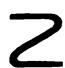
\includegraphics[keepaspectratio]{images/part002_88480e13.jpg}}

例. --- 纯基是超越基。另一方面，若 E 是 K 的一个纯扩张，E 在 K 上的一个超越基不总是 E 的纯基。例如，在 \(\mathbf{K}(\mathbf{X})\) 中， \(\{\mathbf{X}^{2}\}\) 是一个超越基，但不生成 \(\mathbf{K}(\mathbf{X})\) 。

命题7. --- 设 E 是域 K 的一个扩域。 E 的每个超越基都是 E 的在 K 上代数自由的子集所成集合（按包含关系排序）中的极大元。反之，若 S 是 E 的一个子集，使得 E 在 K(S) 上是代数的，则 S 的每个极大代数自由子集都是 E 的一个超越基。

设 B 是 E 在 K 上的一个超越基，且 \(x \in E - B\) 。则 x 在 \(\mathrm{K}(\mathrm{B})\) 上是代数的；由 V 第107页命题4，E 的子集 \(B \cup \{x\}\) 在 K 上不是代数自由的，由此得命题的第一部分。其次，若 E 在 \(\mathrm{K}(\mathrm{S})\) 上代数，且 B 是 S 的一个极大代数自由部分，则由命题4的推论，每个 \(x \in S\) 在 \(\mathrm{K}(\mathrm{B})\) 上是代数的；于是（V，第18页，推论1） \(\mathrm{K}(\mathrm{S})\) 在 \(\mathrm{K}(\mathrm{B})\) 上是代数的，从而（V，第19页，命题3）E 在 \(\mathrm{K}(\mathrm{B})\) 上是代数的。

定理1（施泰尼茨）。--- 域 K 的每个扩域 E 在 K 上都拥有一个超越基。换言之，域 K 的每个扩张都是 K 的一个纯扩张的代数扩张。

\pandocbounded{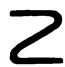
\includegraphics[keepaspectratio]{images/part002_71d10db7.jpg}}

相反，一个扩张并不总是代数扩张的纯扩张（V，第171页，习题2）。

此定理是以下更精确结果的一个推论：

定理2. --- 设 E 是域 K 的一个扩域，S 是 E 的一个使 E 在 K(S) 上代数的子集，T 是 S 的一个在 K 上代数自由的子集；则存在 E 在 K 上的一个超越基 B，使得 \(T \subset B \subset S\) 。

因为 S 的代数自由子集所成的集合按包含关系排序，由命题3是一个有限特征集（E，III，第34页）。由 E，III，第35页的定理1，它有一个包含 T 的极大元 B，且由命题7，B 是 E 在 K 上的一个超越基。

推论（«交换定理»）。--- 设 E 是 K 的一个扩域，S 是 E 的一个使 E 在 K(S) 上代数的子集，T 是 E 的一个在 K 上代数自由的子集；则存在 S 的一个子集 S'，使得 T ∪ S' 是 E 在 K 上的一个超越基，且 T ∩ S' = ∅。

因为 E 在 \(\mathbf{K}(\mathbf{T} \cup \mathbf{S})\) 上是代数的，且我们有 \(T \subset T \cup S\) 。

\subsection{扩张的超越次数}

定理3. --- 设 E 是域 K 的一个扩域。 E 在 K 上的所有超越基都具有相同的基数。

只需证明不等式 \(\operatorname{Card}(\mathbf{B}) \geqslant \operatorname{Card}(\mathbf{B}')\) ，其中 \(\mathbf{B}\) 与 \(\mathbf{B}'\) 是 \(\mathbf{E}\) 在 \(\mathbf{K}\) 上的两个超越基，并且我们可设 \(\mathbf{B}'\) 非空。我们先假设 \(\mathbf{B}\) 有限，并对其基数 \(n\) 作归纳；当 \(n = 0\) 时， \(\mathbf{E}\) 在 \(\mathbf{K}\) 上是代数的，且 \(\mathbf{B}'\) 为空。现设 \(n \geqslant 1\) ；给定 \(x \in \mathbf{B}'\) ，交换定理提供子集 \(\mathbf{C}\) （ \(\mathbf{B}\) 的），使得 \(x \notin \mathbf{C}\) 且 \(\{x\} \cup \mathbf{C}\) 是 \(\mathbf{E}\) 在 \(\mathbf{K}\) 上的一个超越基；由命题7我们有 \(\mathbf{C} \neq \mathbf{B}\) ，因此 \(\operatorname{Card} \mathbf{C} < n\) 。令 \(\mathbf{K}_1 = \mathbf{K}(x)\) 且 \(\mathbf{C}' = \mathbf{B}' - \{x\}\) ；则 \(\mathbf{C}\) 与 \(\mathbf{C}'\) 在域 \(\mathbf{K}_1\) 上代数自由（V，第107页，命题4），且 \(\mathbf{E}\) 既在 \(\mathbf{K}_1(\mathbf{C}) = \mathbf{K}(\mathbf{C} \cup \{x\})\) 上、又在 \(\mathbf{K}_1(\mathbf{C}') = \mathbf{K}(\mathbf{B}')\) 上是代数的。换言之， \(\mathbf{C}\) 与 \(\mathbf{C}'\) 是 \(\mathbf{E}\) 在 \(\mathbf{K}_1\) 上的两个超越基。由于 \(\operatorname{Card}(\mathbf{C}) < n\) ，归纳假设给出不等式 \(\operatorname{Card}(\mathbf{C}') \leqslant \operatorname{Card}(\mathbf{C}) \leqslant n - 1\) ，从而 \(\operatorname{Card}(\mathbf{B}') \leqslant n = \operatorname{Card}(\mathbf{B})\) 。

现设 B 是无限的。每个 \(x \in B\) 在 \(\mathrm{K}(\mathrm{B}')\) 上是代数的，于是存在有限子集 \(\mathrm{S}(x)\) （ \(B'\) 的），使得 x 在 \(\mathrm{K}(\mathrm{S}(x))\) 上是代数的。记 \(\mathrm{S} = \bigcup_{x \in \mathrm{B}} \mathrm{S}(x)\) ，则 \(S \subset B'\) ，且由于 B 是无限的，我们有 \(\operatorname{Card}(\mathrm{S}) \leqslant \operatorname{Card}(\mathrm{B})\)

（E，III，第49页，推论3）。但由于 B 的每个元素在 K(S) 上是代数的，且 E 在 K(B) 上是代数的，我们得出 E 在 K(S) 上是代数的（V，第19页，命题3）。现在命题7蕴含 S = B'，从而得到所希望的不等式 Card(B') ≤ Card(B)。

定义4. --- 设 E 是域 K 的一个扩域。 E 在 K 上的每个超越基的基数称为 E 在 K 上的超越次数，记作 tr. deg \(_{K}\) E。

定理2、定理3以及定义4蕴含以下推论，其中 E 表示域 K 的一个具有有限超越次数 n 的扩域。

推论1. --- 设 S 是 E 的一个子集，使得 E 在 K(S) 上是代数的。则 Card(S) ≥ n；若 S 的基数等于 n，则 S 在 K 上是代数自由的（从而此时它是 E 在 K 上的一个超越基）。

推论2. --- 假设 \(\mathrm{E} = \mathrm{K}(x_1, \ldots, x_m)\) ，则 \(m \geqslant n\) ；此外若 \(m = n\) ，则 \((x_1, \ldots, x_m)\) 是 \(\mathrm{E}\) 在 \(\mathrm{K}\) 上的一个纯基，从而 \(\mathrm{E}\) 是 \(\mathrm{K}\) 的一个纯扩张。

推论3. --- E 的每个在 K 上代数自由的子集至多有 n 个元素，若它恰好有 n 个元素，则它是 E 在 K 上的一个超越基。

定理4. --- 设 K、E 和 F 是三个域，满足 \(K \subset E \subset F\) 。若 S 是 E 在 K 上的一个超越基，T 是 F 在 E 上的一个超越基，则 \(S \cap T\) 为空，且 \(S \cup T\) 是 F 在 K 上的一个超越基。

因为 F 在 \(E(T)\) 上是代数的；此外， \(E(T)\) 在域 \(K(S \cup T) = K(S)(T)\) 上是代数的，因为 E 在 \(K(S)\) 上是代数的（V，第18页，推论2）；因此（V，第19页，命题3）F 在 \(K(S \cup T)\) 上是代数的。另一方面，T 在 E 上代数自由，从而在 \(K(S)\) 上更是如此，故（V，第107页，命题4） \(S \cup T\) 在 K 上代数自由，且 \(S \cap T = \varnothing\) 。

推论. --- 设 K、E 和 F 是三个域，满足 \(K \subset E \subset F\) 。则我们有

\[
\operatorname{tr} \cdot \deg_ {K} F = \operatorname{tr} \cdot \deg_ {K} E + \operatorname{tr} \cdot \deg_ {E} F.\tag{1}
\]

\subsection{同构的扩张}

命题8. --- 设 \(\Omega\) 是域 K 的一个代数闭扩张，E 和 F 是 \(\Omega\) 的两个子扩张， \(u\) 是 E 到 F 上的一个 K-同构。为使一个 K-自同构 \(v\) （ \(\Omega\) 的、且延拓 \(u\) ）存在，充要条件是 \(\Omega\) 在 E 与 F 上具有相同的超越次数。

该条件显然是必要的。

现设 \(\Omega\) 在 E 和 F 上具有相同的超越次数，并选取 \(\Omega\) 在 E 上的一个超越基 B 以及 \(\Omega\) 在 F 上的一个超越基 C。由于 B 与 C 等势，命题2（V，第106页）表明 \(u\) 可扩张为 E(B) 到 F(C) 上的一个 K-同构 \(u'\) 。由于 \(\Omega\) 是 E(B) 与 F(C) 的代数闭包，V 第23页的推论表明 \(u'\) 可扩张为一个自同构 \(v\) （ \(\Omega\) 的）。

推论1. --- 设 \(\Omega\) 是域 K 的一个代数闭扩张，E 是 \(\Omega\) 的一个子扩张。 E 的每个 K-自同构都可扩张为 \(\Omega\) 的一个 K-自同构。

推论2. --- 设 \(\Omega\) 是域 \(K\) 的一个代数闭扩张， \(E\) 与 \(F\) 是 \(\Omega\) 的两个子扩张， \(u\) 是 \(E\) 到 \(F\) 上的一个 K-同构。若 \(E\) 在 \(K\) 上的超越次数有限（特别地，若 \(E\) 在 \(K\) 上是代数的），则存在 \(\Omega\) 的一个延拓 \(u\) 的 K-自同构。

我们用 n、 \(d(\mathrm{E})\) 与 \(d(\mathrm{F})\) 分别表示 E 在 K 上的、 \(\Omega\) 在 E 上的以及 \(\Omega\) 在 F 上的超越次数。 K-同构 u 的存在性表明 F 在 K 上的超越次数等于 n。由定理4的推论， \(\Omega\) 在 K 上的超越次数等于 \(d(\mathrm{E}) + n\) ，也等于 \(d(\mathrm{F}) + n\) 。因此（E，III，第28页，命题8）我们有 \(d(\mathrm{E}) = d(\mathrm{F})\) ，从而可以应用命题8。

命题9. --- 设 K 是一个域， \(\Omega\) 是 K 的一个代数闭扩张。假设 \(\Omega\) 在 K 上不是代数的；则 \(\Omega\) 中在 K 上超越的元素所成的集合是无限的。此外，若 \(x\) 与 \(y\) 是 \(\Omega\) 的两个在 K 上超越的元素，则存在一个自同构 \(u\) （ \(\Omega\) 的、在 K 上的），使得 \(u(x) = y\) 。

由于 \(\Omega\) 在 \(\mathbf{K}\) 上不是代数的，存在一个元素 \(x\) （ \(\Omega\) 的、在 \(\mathbf{K}\) 上超越的）；于是元素 \(x^n\) （ \(n \in \mathbf{N}\) ）两两不同且在 \(\mathbf{K}\) 上超越。设 \(x\) 与 \(y\) 不同且在 \(\mathbf{K}\) 上超越；由命题2（V，第106页），存在一个 K-同构 \(\tilde{u}\) ，从 \(\mathbf{K}(x)\) 到 \(\mathbf{K}(y)\) 上，使得 \(\tilde{u}(x) = y\) ；由于 \(\mathbf{K}(x)\) 在 \(\mathbf{K}\) 上的超越次数为 1，命题8的推论2表明 \(\tilde{u}\) 可扩张为一个 K-自同构 \(u\) （ \(\Omega\) 的）。

命题10. --- 设 K 是一个域，Ω 是 K 的一个代数闭扩张，G 是 Ω 的 K-自同构群。设 \(x \in \Omega\) 。

\begin{enumerate}
\def\labelenumi{\alph{enumi})}
\item
  为使 \(x\) 在 \(K\) 上是代数的，充要条件是：元素 \(u(x)\) （当 \(u\) 取遍 \(G\) ）所成的集合是有限的，
\item
  为使 \(x\) 是 \(p\) -根式的（相对于 \(\mathbf{K}\) ），充要条件是 \(u(x) = x\) （对所有 \(u \in \mathbf{G}\) ）成立。
\end{enumerate}

特别地，若 K 是完全域，则群 G 的不变量集合等于 K。首先设 x 是超越的。由命题9， \(\Omega\) 中在 K 上超越的元素所成的集合 T 是无限的，且对每个 \(y \in T\) ，存在 \(u \in G\) 使得 \(u(x) = y\) 。因此，当 u 取遍 G 时元素 \(u(x)\) 所成的集合是无限的。

现设 \(x\) 在 \(\mathbf{K}\) 上是代数的，并用 \(f\) 表示它在 \(\mathbf{K}\) 上的极小多项式； \(f\) 在 \(\Omega\) 中的根所成的集合是有限的，且对每个 \(u \in \mathbf{G}\) 我们有 \(f(u(x)) = u(f(x)) = 0\) 。因此，元素 \(u(x)\) （当 \(u\) 取遍 \(\mathbf{G}\) ）所成的集合是有限的。这就证明了 \(a\) 。

设 L 为 \(\Omega\) 中满足 \(u(y)=y\) （对所有 \(u\in G\) ）的元素 y 组成的集合，并设 \(\bar{K}\) 为 K 在 \(\Omega\) 中的相对代数闭包。由上所述，L 是 \(\bar{K}\) 在 K 上的一个子扩张。此外（命题8的推论1）， \(\bar{K}\) 的每个 K-自同构都是 G 的某个元素在 \(\bar{K}\) 上的限制。命题10的断言 b) 现由 V 第53页的推论3得出。

\subsection{代数不相交扩张}

定义5. --- 设 L 是域 K 的一个扩域，E 和 F 是 L 的两个子扩张。若对于 E（相应地，F）的每个在 K 上代数自由的子集 A（相应地，B），A 与 B 不相交且 A ∪ B 在 K 上代数自由，则称 E 与 F（在 K 上）代数不相交，并称 E 在 K 上与 F 代数不相交。

注记. --- 1) 若 E 是 L 的一个子扩张，且在 K 上是代数的，则它与 L 的每个子扩张 F 都是代数不相交的。一个 K 的扩张是代数的，当且仅当它与自身代数不相交。

\begin{enumerate}
\def\labelenumi{\arabic{enumi})}
\setcounter{enumi}{1}
\item
  可能发生 E 在 K 上与 F 代数不相交、但在 K 的某个子域 \(K_{0}\) 上并非如此的情形。* 例如，C 在 R 上与自身代数不相交，但在 Q 上并非如此。*
\item
  显然，如果 E 在 K 上与 F 代数不相交，那么当 E 和 F 被视为 L 的子扩张时，这一性质在它们被视为 \(\mathbf{K}(\mathbf{E} \cup \mathbf{F})\) 的子扩张时同样成立，反之亦然。
\end{enumerate}

命题11. --- 若E与F在K上代数不相交，则E ∩ F在K上是代数的。

这由定义5得出。

命题12. --- 设L是域K的一个扩域，E、F是L的子扩域。则以下条件等价：

\begin{enumerate}
\def\labelenumi{\alph{enumi})}
\item
  E 与 F 代数不相交；
\item
  存在 E 在 K 上的一个超越基，它在 F 上是代数自由的。
\item
  E 的每个在 K 上代数自由的子集都在 F 上代数自由。我们引入以下条件：
\end{enumerate}

\(b^{\prime})\) 存在 \(\mathbf{F}\) 在 \(\mathbf{K}\) 上的一个超越基，它在 \(\mathbf{E}\) 上代数自由；

\(c^{\prime})\) \(\mathbf{F}\) 的每个在 \(\mathbf{K}\) 上代数自由的子集都在 \(\mathbf{E}\) 上代数自由。

\(a) \Rightarrow b')\) ：设 E 与 F 代数不相交。设 B（相应地，C）是 E（相应地，F）在 K 上的一个超越基。则 \(B \cap C = \emptyset\) 且 \(B \cup C\) 在 K 上代数自由，因此 C 在 \(K(B)\) 上代数自由（V，第107页，命题4）；由于 E 在 \(K(B)\) 上是代数的，V 第108页的命题6表明 C 在 E 上代数自由。

\(b') \Rightarrow c)\) ：假设存在 F 在 K 上的一个超越基 C，且 C 在 E 上是代数自由的。设 A 是 E 的一个在 K 上代数自由的子集。则 C 在 K(A) 上是代数自由的，因此 A 在 K(C) 上是代数自由的（V，第107页，命题4），从而在 F 上也是代数自由的（V，第108页，命题6），因为 F 在 K(C) 上是代数的。

\(c) \Rightarrow a)\) 这由命题4（V，第107页）立即得出。

蕴含关系 \(a) \Rightarrow b) \Rightarrow c') \Rightarrow a)\) 可以用同样的方式证明。

推论. --- 设 E 与 F 在 K 上代数不相交。设 E' 为 E 在 L 中的相对代数闭包，F' 为 F 在 L 中的相对代数闭包（V，第19页）。则 E' 与 F' 在 K 上代数不相交。

设 B 是 E 在 K 上的一个超越基；它也是 \(E'\) 在 K 上的一个超越基。由于 E 在 K 上与 F 代数不相交，B 在 F 上代数自由，从而在 \(F'\) 上代数自由（V，第108页，命题6）；于是可以应用命题12。

命题 13. --- 设 L 是域 K 的一个扩张，且 E、F 是 L 的两个子扩张。

\begin{enumerate}
\def\labelenumi{\alph{enumi})}
\tightlist
\item
  我们有 \(\operatorname{tr} \cdot \deg_{\mathbb{F}} \mathrm{F}(\mathrm{E}) \leqslant \operatorname{tr} \cdot \deg_{\mathbb{K}} \mathrm{E}\) 。当 \(\mathrm{E}\) 与 \(\mathrm{F}\) 在 \(\mathbf{K}\) 上代数不相交时， \(\mathrm{E}\) 在 \(\mathbf{K}\) 上的每个超越基都是
\end{enumerate}

\(F(E)\) 在 F 上的一个超越基，并且我们有 tr. \(\deg_{F}F(E) = \text{tr. } \deg_{K}E\) 。反之，这个等式蕴含 E 与 F 在 K 上代数不相交，当 tr. \(\deg_{K}E\) 有限时。

\begin{enumerate}
\def\labelenumi{\alph{enumi})}
\setcounter{enumi}{1}
\item
  我们有 \(\operatorname{tr} \cdot \deg_{\mathbf{K}} \mathrm{K}(\mathrm{E} \cup \mathrm{F}) \leqslant \operatorname{tr} \cdot \deg_{\mathbf{K}} \mathrm{E} + \operatorname{tr} \cdot \deg_{\mathbf{K}} \mathrm{F}\) 。当 \(\mathrm{E}\) 与 \(\mathrm{F}\) 在 \(\mathbf{K}\) 上代数不相交时，我们有 \(\operatorname{tr} \cdot \deg_{\mathbf{K}} \mathrm{K}(\mathrm{E} \cup \mathrm{F}) = \operatorname{tr} \cdot \deg_{\mathbf{K}} \mathrm{E} + \operatorname{tr} \cdot \deg_{\mathbf{K}} \mathrm{F}\) 。反之，这个等式蕴含 \(\mathrm{E}\) 与 \(\mathrm{F}\) 在 \(\mathbf{K}\) 上代数不相交，当 \(\mathrm{E}\) 与 \(\mathrm{F}\) 在 \(\mathbf{K}\) 上超越次数有限时。
\item
  设 B 是 E 在 K 上的一个超越基；则 E 在 K(B) 上是代数的，且 V 第18页的推论2表明 F(E) 在 F(K(B)) = F(B) 上是代数的。由定理2（V，第109页），B 包含 F(E) 在 F 上的一个超越基；当 E 在 K 上与 F 代数不相交时，B 在 F 上是代数自由的（命题12），此时它就是 F(E) 在 F 上的一个超越基。a) 的前三个断言由此得出。现设 E 在 K 上的超越次数有限，且等于 F(E) 在 F 上的超越次数；由于 F(E) 在 F(B) 上是代数的且 Card B = tr . deg\_F F(E)，V 第110页的推论1表明 B 在 F 上是代数自由的，因此 E 在 K 上与 F 代数不相交（命题12）。
\item
  我们有 \(\mathbf{K}(\mathbf{E} \cup \mathbf{F}) = \mathbf{F}(\mathbf{E})\) ，从而 V 第 110 页的推论蕴含等式：
\end{enumerate}

\[
\operatorname{tr} \cdot \deg_ {K} K (E \cup F) = \operatorname{tr} \cdot \deg_ {F} F (E) + \operatorname{tr} \cdot \deg_ {K} F.
\]

现在 \(b)\) 立即由 \(a)\) 及此等式得出。

命题14. --- 设 L 是域 K 的一个扩域，E 和 F 是 L 的两个子扩张，且 B 是 E 在 K 上的一个超越基。为使 E 与 F 在 K 上代数不相交，充要条件是 K(B) 与 F 在 K 上线性不相交。

为使 E 与 F 在 K 上代数不相交，充要条件是 B 在 F 上代数自由（命题12），即 B 中元素的单项式在 F 上线性无关。由于这些单项式构成向量 K-空间 K{[}B{]} 的一组基，这等价于说 K{[}B{]} 与 F 在 K 上线性不相交。最后，由于 K(B) 是 K{[}B{]} 的分式域，V 第14页的命题6表明 K{[}B{]} 与 F 线性不相交当且仅当 K(B) 与 F 线性不相交。

推论1. --- 若 E 与 F 线性不相交，则 E 在 K 上与 F 代数不相交。反之，若 E 是 K 的一个纯扩张，且在 K 上与 F 代数不相交，则 E 与 F 在 K 上线性不相交。

推论2. --- K 的每个纯扩张与 K 的每个代数扩张都线性不相交；特别地，K 在 K 的每个纯扩张中都是相对代数闭的。

\subsection{扩张的代数自由族}

定义6. --- 设 L 是域 K 的一个扩域， \((\mathrm{E}_{i})_{i\in I}\) 是 L 的子扩张的一个族。族 \((\mathrm{E}_{i})_{i\in I}\) 称为代数自由的，如果下列条件满足：

(AF) 对每个 \(i \in I\) ，设 \(\mathbf{A}_i\) 是 \(\mathbf{E}_i\) 的一个在 \(\mathbf{K}\) 上代数自由的子集。则 \(\mathbf{A}_i \cap \mathbf{A}_j = \emptyset\) （对 \(i \neq j\) ），且 \(\cup \mathbf{A}_i\) 在 \(\mathbf{K}\) 上代数自由。

注记. --- 由命题3（V，第107页），只需对有限子集 \(A_{i}\) 验证条件（AF）即可。由此我们得到如下结果：若 \((\mathrm{E}_{i})_{i\in I}\) 是代数自由族，则 \((\mathrm{E}_{i}^{\prime})_{i\in I}\) 亦然，只要 \(E_{i}^{\prime}\) 是 \(E_{i}\) 的一个子扩张（对每个 \(i\in I\) ）；反之，若每个族 \((\mathrm{E}_{i}^{\prime})_{i\in I}\) （其中 \(E_{i}^{\prime}\) 是 E 的一个有限生成子扩张，对每个 \(i\in I\) ）都是代数自由的，则 \((\mathrm{E}_{i})_{i\in I}\) 是代数自由的。另一方面，为使 \((\mathrm{E}_{i})_{i\in I}\) 是代数自由的，充要条件是 \((\mathrm{E}_{i})_{i\in J}\) 对 I 的每个有限子集 J 都是代数自由的。直观地可以说，扩张的代数无关性是一种“有限特征”的性质。

命题15. --- 设 \((\mathbf{E}_i)_{i\in I}\) 是域 K 的一个给定扩张 L 的子扩张族。则下列条件等价：

\begin{enumerate}
\def\labelenumi{\alph{enumi})}
\item
  族 \((\mathrm{E}_i)_{i\in I}\) 是代数自由的。
\item
  对每个 \(i \in I\) ，扩张 \(E_i\) 在 \(K\) 上与扩张 \(F_i\) （由诸 \(E_j\) （ \(j \neq i\) ）生成的）代数不相交。
\item
  存在一个族 \((\mathbf{B}_i)_{i\in I}\) （由 \(L\) 的两两不相交的子集组成），使得 \(\mathbf{B}_i\) 是 \(\mathbf{E}_i\) 在 \(K\) 上的一个超越基（对每个 \(i\in I\) ），且 \(\mathbf{B} = \bigcup_{i\in I}\mathbf{B}_i\) 在 \(K\) 上代数自由。
\end{enumerate}

显然 \(a)\) 蕴含 \(c)\) 。

假设 \(c\) )，我们选取 \(i\) （属于 \(I\) ）；令 \(C_i = \bigcup_{j \neq i} B_j\) 。对每个 \(j \neq i\) ，每个元素

（属于 \(E_{j}\) 的）在 \(\mathbf{K}(\mathbf{B}_{j})\) 上是代数的，从而在 \(\mathbf{K}(\mathbf{C}_{i})\) 上更是如此。由 V 第18页的推论1，域 \(F_{i}\) 因此在 \(\mathbf{K}(\mathbf{C}_{i})\) 上是代数的。此外，我们有 \(B_{i} \cap C_{i} = \varnothing\) 且 \(B = B_{i} \cup C_{i}\) 在 K 上代数自由；因此 \(B_{i}\) 在 \(\mathbf{K}(\mathbf{C}_{i})\) 上代数自由（V，第107页，命题4），从而也在 \(F_{i}\) 上代数自由（它在 \(\mathbf{K}(\mathbf{C}_{i})\) 上是代数的），由 V 第108页的命题6。于是我们证明了 \(E_{i}\) 在 K 上与 \(F_{i}\) 代数不相交（V，第113页，命题12），故 c) 蕴含 b)。

现在假设 \(b)\) 并证明 \(a)\) 。只需证明：若 \(i_1, \ldots, i_n\) 是 \(I\) 中互不相同的元素，则扩张族 \((E_{i_1}, \ldots, E_{i_n})\) 是代数自由的；我们对 \(n\) 作归纳论证，情形 \(n = 1\) 是平凡的。现设 \(n > 1\) 且族 \((E_{i_1}, \ldots, E_{i_{n-1}})\) 是代数自由的；对 \(1 \leqslant k \leqslant n\) ，选取一个子集 \(A_k\) （ \(E_{i_k}\) 的、在 \(K\) 上代数自由的），并设

\(B = A_{1} \cup \ldots \cup A_{n-1}\) 。由归纳假设，子集 \(A_{1}, \ldots, A_{n-1}\) 两两不相交，且 B 在 K 上代数自由；由 b)， \(E_{i_{n}}\) 与 \(F_{i_{n}}\) 代数不相交，且由于 B 包含于 \(F_{i_{n}}\) ，我们有 \(B \cap A_{n} = \varnothing\) 且 \(B \cup A_{n} = A_{1} \cup \ldots \cup A_{n}\) 在 K 上代数自由。于是我们证明了族 \((E_{i_{1}}, \ldots, E_{i_{n}})\) 是代数自由的。

下面的命题推广了命题13（V，第113页）的 \(b)\) 部分。

命题16. --- 设 \((\mathrm{E}_i)_{i\in I}\) 是域 K 的一个扩张的子扩张族，并设 E 是由 \(\cup\) \(\mathrm{E}_i\) 生成的域。

\begin{enumerate}
\def\labelenumi{\alph{enumi})}
\item
  我们有 \(\operatorname{tr} \cdot \deg_{\mathbf{K}} \mathrm{E} \leqslant \sum_{i \in I} \operatorname{tr} \cdot \deg_{\mathbf{K}} \mathrm{E}_i\) ，并且当族 \((\mathrm{E}_i)_{i \in I}\) 在 \(\mathbf{K}\) 上代数自由时取等号。
\item
  反之，假设 \(\operatorname{tr} \cdot \deg_{\mathbf{K}} \mathrm{E} = \sum_{i \in I} \operatorname{tr} \cdot \deg_{\mathbf{K}} \mathrm{E}_i\) 且 \(\operatorname{tr} \cdot \deg_{\mathbf{K}} \mathrm{E}\) 有限；则族 \((\mathrm{E}_i)_{i \in I}\) 在 \(\mathbf{K}\) 上代数自由。
\end{enumerate}

对每个 \(i \in I\) ，设 \(\mathbf{B}_i\) 是 \(\mathbf{E}_i\) 在 \(\mathbf{K}\) 上的一个超越基，并设 \(\mathbf{B} = \bigcup_{i \in I} \mathbf{B}_i\) 。对每个 \(i \in I\) ， \(\mathbf{E}_i\) 的每个元素在 \(\mathbf{K}(\mathbf{B}_i)\) 上是代数的，从而在

K(B) 上是代数的。现在 V 第18页的推论1表明 E 在 K(B) 上是代数的；由 V 第109页定理2，B 包含 E 在 K 上的一个超越基。此外，若族 \((\mathrm{E}_{i})_{i\in I}\) 在 K 上是代数自由的，则诸 \(B_{i}\) 两两不相交，且集合 B 在 K 上代数自由。这就建立了 a)（集合论，III，第160页，命题4的推论）。

在 \(b\) ) 的假设下，E 在 \(\mathbf{K}(\mathbf{B})\) 上是代数的，且在 \(\mathbf{K}\) 上超越次数有限，并且我们有 \(\operatorname{Card}(\mathbf{B}) \leqslant \operatorname{tr} \cdot \deg_{\mathbf{K}} \operatorname{E}\) 。由 V 第110页的推论1，B 在 \(\mathbf{K}\) 上代数自由，且诸 \(\mathbf{B}_i\) 两两不相交。现在命题15表明族 \((\mathrm{E}_i)_{i \in I}\) 在 \(\mathbf{K}\) 上代数自由。

在陈述下一个定理之前，我们指出存在具有任意超越次数的 K 的代数闭扩张，例如一个适当的有理分式域的代数闭包。

定理5. --- 设 \((\mathrm{E}_i)_{i\in I}\) 是域 \(\mathbf{K}\) 的一族扩张， \(\Omega\) 是 \(\mathbf{K}\) 的一个代数闭扩张。假设不等式

\[
\operatorname{tr} \cdot \deg_ {K} \Omega \geqslant \sum_ {i \in I} \operatorname{tr} \cdot \deg_ {K} E _ {i}\tag{2}
\]

成立。则存在一个代数自由族 \((\mathrm{F}_i)_{i\in I}\) （由 \(\Omega\) 的子扩张组成），使得 \(\mathbf{F}_i\) 与 \(\mathbf{E}_i\) 是 K-同构的（对所有 \(i\in I\) ）。

对每个 \(i \in I\) ，设 \(B_i\) 是 \(E_i\) 在 \(K\) 上的一个超越基。设 \(B\) 是 \(\Omega\) 在 \(K\) 上的一个超越基。由 (2) 我们有 Card \(B \geqslant \sum_{i \in I} \text{Card } B_i\) ；因此

存在 B 的两两不相交子集的一个族 \((\mathbf{B}_{i}^{\prime})_{i\in I}\) 以及双射 \(u_{i}:B_{i}\to B_{i}^{\prime}\) （对 \(i\in I\) ）。由 V 第106页的命题2， \(u_{i}\) 扩张为一个 K-同构 \(v_{i}\) （从 \(\mathbf{K}(\mathbf{B}_{i})\) 到 \(\mathbf{K}(\mathbf{B}_{i}^{\prime})\) 上的）；由于 \(\Omega\) 是代数闭的且 \(E_{i}\) 在

\(K(B_{i})\) 上是代数的，推论（V，第23页）表明 \(v_{i}\) 延拓为 \(E_{i}\) 到一个子扩张 \(F_{i}\) （ \(\Omega\) 的）上的一个 K-同构。根据构造， \(B_{i}^{\prime}\) 是 \(F_{i}\) 在 K 上的一个超越基，且命题15（V，第115页）表明子扩张族 \((F_{i})_{i\in I}\) （ \(\Omega\) 的）在 K 上是代数自由的。

推论1. --- 设 E 和 Ω 是域 K 的两个扩张。假设 Ω 是代数闭的，其超越次数至少等于 E 的超越次数。则 E 与 Ω 的一个子扩张是 K-同构的。

推论2. --- 设 \(\Omega\) 是一个在其素子域上具有无限超越次数的代数闭域。则每个与 \(\Omega\) 特征相同的域都是同构于 \(\Omega\) 的子域的域的上升有向并。

因为每个域都是其素域上有限生成的子域的上升有向并，于是只需应用推论1即可。

* 例. --- 这特别适用于特征 0 的情形，即取 \(\Omega = \mathbf{C}\) （“莱夫谢茨原理”）。 *

\subsection{有限生成扩张}

命题17. --- 设 E 是域 K 的一个扩域，B 是 E 在 K 上的一个超越基。为使 E 在 K 上是有限生成的（V，第11页，定义2），充要条件是 B 有限且次数 {[}E : K(B){]} 有限。

设 E 在 K 上是有限生成的，并设 S 是 E 的一个有限子集，使得 \(\mathrm{E} = \mathrm{K}(\mathrm{S})\) 。由定理2（V，第109页），S 包含 E 在 K 上的一个超越基 \(B'\) ，且它与 B 有相同的基数（V，第110页，定理3）。因此 B 是有限的。设 \(\mathrm{K}' = \mathrm{K}(\mathrm{B})\) ；则 E 在 \(K'\) 上是代数的，且我们有 \(\mathrm{E} = \mathrm{K}'(\mathrm{S})\) ；由于 S 有限，V 第18页的定理2表明 \([E : K']\) 是有限的。

反之，设 B 有限且 \([E:K(B)]\) 有限。若 C 是向量空间 E 在 \(K(B)\) 上的一个（有限）基，则我们有 \(E = K(B)(C) = K(B \cup C)\) ，于是 E 是 K 的一个有限生成扩张。

推论1. --- 设 E 是 K 的一个有限生成扩张，并设 K' 是 K 在 E 中的相对代数闭包（V，第19页）。则 K' 在 K 上是有限次的。

设 B 是 E 在 K 上的一个超越基。由 V 第114页的推论2， \(K'\) 与 \(\mathrm{K}(\mathrm{B})\) 在 K 上线性不相交，因此 \([\mathrm{K}' : \mathrm{K}] = [\mathrm{K}'(\mathrm{B}) : \mathrm{K}(\mathrm{B})] \leq [\mathrm{E} : \mathrm{K}(\mathrm{B})]\) ，于是 \([\mathrm{K}' : \mathrm{K}]\) 的有限性由 \([\mathrm{E} : \mathrm{K}(\mathrm{B})]\) 的有限性得出。

推论2. --- 一个在其素子域上有限生成的域只包含有限多个单位根。

由推论1，我们归结为证明：一个域 L，若它是其素子域的有限次扩张，则只含有有限多个单位根。当 L 的特征 \(\neq0\) 时这是显然的，因为此时它是有限的。若 L 的特征为 0 且包含无穷多个单位根，则它包含任意高阶的本原单位根。由 V 第84页定理2，因此存在无穷多个整数 n \textgreater{} 0 使得 \(\varphi(n) \leqslant [L : Q]\) ，这是荒谬的（V，第80页，公式（2）和（3））。

推论3. --- 若 E 是域 K 的一个有限生成扩张，则 E 的每个子扩张 E' 都是有限生成的。

设 \(B'\) 是 \(E'\) 在 \(K\) 上的一个超越基。由 \(V\) 第109页定理2， \(B'\) 包含于一个超越基 \(B\) （ \(E\) 在 \(K\) 上的）中，因而由命题17是有限的。由于 \(E'\) 在 \(K(B')\) 上是代数的，且 \(E\) 是 \(K(B')\) 的一个有限生成扩张，推论1表明 \([E': K(B')]\) 有限。现在命题17表明 \(E'\) 在 \(K\) 上是有限生成的。

命题17可以用如下方式转述：K 的一个有限生成扩张是纯超越扩张 \(\mathrm{K}(x_{1},\ldots,x_{n})\) 的一个有限次代数扩张。

\section{可分扩张}

\subsection{环的幂零元的刻画}

命题1. --- 设 A 是一个交换环，x 是 A 的一个元素。为使 x 是幂零的，充要条件是 1 - xT 在环 A{[}T{]} 中可逆。

我们注意到 A{[}T{]} 是形式幂级数环 A{[}{[}T{]}{]} 的一个子环，且 1 - xT 在 A{[}{[}T{]}{]} 中有逆元 \(\sum_{n=0}^{\infty} x^{n} T^{n}\) （IV，第30页，命题5）。为使 1 - xT

在 A{[}T{]} 中可逆，充要条件是 \(\sum_{n=0}^{\infty} x^n T^n\) 是一个多项式，

即 \(x\) 是幂零的。

命题2. --- 设 A 是一个交换环。 A 的幂零元集合是 A 的一个理想，等于 A 的所有素理想的交集。

设 \(x\) 是 \(\mathbf{A}\) 的一个幂零元， \(\mathfrak{p}\) 是 \(\mathbf{A}\) 的一个素理想。 \(x \mod \mathfrak{p}\) 的剩余类是整环 \(\mathbf{A} / \mathfrak{p}\) 的一个幂零元，因而是零；于是我们有 \(x \in \mathfrak{p}\) 。

设 \(x\) 是 \(A\) 的一个非幂零元。由命题1，主理想 \((1 - xT)\) （ \(A[T]\) 的）异于 \(A[T]\) 。由 Krull 定理（I，第104页），存在一个极大理想 \(m\) （ \(A[T]\) 的），它包含 \(1 - xT\) 。于是 \(m\) 是 \(A[T]\) 的素理想，因此 \(p = A \cap m\) 是 \(A\) 的素理想。我们有 \(1 \notin m\) 且 \(1 - Tx \in m\) ，因此 \(Tx \notin m\) ，从而 \(x \notin p\) 。

于是我们证明了，A 的幂零元集合 n 是 A 的所有素理想的交集；由于理想的任意交仍是理想，故 n 是一个理想。

推论. --- 为使一个交换环是既约的（V，第34页，定义2），充要条件是它同构于一个域的乘积的子环。

该条件显然是充分的。

设 A 是既约的。由命题2，A 的素理想集合的交 n 化为 0。对 A 的每个素理想 p，设 \(k(\mathfrak{p})\) 是 A/p 的分式域， \(\varphi_{p}\) 是 A 到 \(k(\mathfrak{p})\) 的典范同态。设 \(\varphi\) 是 A 到 \(\prod_{\mathfrak{p}} k(\mathfrak{p})\) 的同态，其指标为 p 的分量是 \(\varphi_{p}\) 。 \(\varphi_{\mathfrak{p}}\) 的核是 \(\mathfrak{p}\) ，故 \(\varphi\) 的核是 \(\mathfrak{n} = 0\) ；因此 \(\varphi\) 是 \(\mathbf{A}\) 到 \(\prod_{\mathfrak{p}} k(\mathfrak{p})\) 的一个子环上的同构。

\subsection{可分代数}

定义1. --- 设 A 是域 K 上的一个交换代数。若对 K 的每个扩张 L，环 L ⊗K A 都是既约的，则称 A 在 K 上是可分的，或称为可分 K-代数。

每个可分代数显然是既约的。部分逆命题见定理3（V，第125页）。

例. --- 1) 设 A 是一个多项式代数 \(K[X_{i}]_{i \in I}\) 。对 K 的每个扩张 L，环 \(L \otimes_{K} A\) 同构于 \(L[X_{i}]_{i \in I}\) （III，第449页，注记2），因此是一个整环（IV，第9页，命题8）。换言之，域 K 上的每个多项式代数都是可分 K-代数。

\begin{enumerate}
\def\labelenumi{\arabic{enumi})}
\setcounter{enumi}{1}
\item
  设 A 是域 K 上的一个有限次交换代数。为使 A 是可分的，充要条件是它是平展的（V，第34页，定理4）。
\item
  设 E 是域 K 的一个代数扩张。若 L 是 K 的一个扩张，则环 \(L \otimes_{K} E\) 是子环 \(L \otimes_{K} F\) 的并，其中 F 遍历 E 的所有有限次子扩张；因此环 \(L \otimes_{K} E\) 是既约的当且仅当对 E 的每个在 K 上有限的子扩张 F， \(L \otimes_{K} F\) 都是既约的。顾及例2，我们看到 E 是上述定义1意义下的可分代数，当且仅当它是 V 第36页定义1意义下的可分代数扩张。
\end{enumerate}

命题3. --- 设K是一个域。

\begin{enumerate}
\def\labelenumi{\alph{enumi})}
\item
  可分 K-代数的每个子代数都是可分的。
\item
  可分 K-代数的每个直接极限都是可分的。
\item
  可分 K-代数的每个乘积都是可分的。
\item
  设 A 是一个 K-代数， \(K'\) 是 K 的一个扩张。为使 A 是可分的，充要条件是由 A 经标量扩张得到的 \(K'\) -代数 \(\mathbf{A}_{(\mathbf{K}')}\) 是可分的。
\end{enumerate}

设 \(\mathbf{L}\) 是 \(\mathbf{K}\) 的一个扩张。设 \(\mathbf{A}\) 是 \(\mathbf{K}\) 上的一个可分代数， \(\mathbf{B}\) 是 \(\mathbf{A}\) 的一个子代数；则环 \(\mathbf{L} \otimes_{\mathbf{K}} \mathbf{A}\) 是既约的，且 \(\mathbf{L} \otimes_{\mathbf{K}} \mathbf{B}\) 同构于 \(\mathbf{L} \otimes_{\mathbf{K}} \mathbf{A}\) 的一个子环，因而是既约的。于是 \(\mathbf{B}\) 是可分的，这就证明了 \(a)\) 。同理可证 \(b)\) ，利用 \(L \otimes_{K} \varinjlim A_i\) 与 \(\varinjlim L \otimes_K A_i\) 的典范同构（II，第290页，命题7）；而 \(c)\) 由指出 \(L \otimes_K \left( \prod_{i \in I} A_i \right)\) 同构于 \(\prod_{i \in I} (L \otimes_K A_i)\) 的一个子环（II，第306页，命题15）得到证明。

我们将使用 \(d\) ) 的记号。对每个扩张 \(\mathbf{L}'\) （ \(\mathbf{K}'\) 的），环 \(\mathbf{L}' \otimes_{\mathbf{K}'} \mathbf{A}_{(\mathbf{K}')}\) 与 \(\mathbf{L}' \otimes_{\mathbf{K}} \mathbf{A}\) 是同构的（II，第278页，命题2）。我们得出结论：若 \(\mathbf{A}\) 是可分 \(\mathbf{K}\) -代数，则 \(\mathbf{A}_{(\mathbf{K}')}\) 是可分 \(\mathbf{K}'\) -代数。反之，设 \(\mathbf{A}_{(\mathbf{K}')}\) 是可分 \(\mathbf{K}'\) -代数；前面的注记表明 \(\mathbf{L}' \otimes_{\mathbf{K}} \mathbf{A}\) 是既约的（对每个扩张 \(\mathbf{L}'\) （ \(\mathbf{K}\) 的、包含 \(\mathbf{K}'\) 作为子扩张））。设 \(\mathbf{L}\) 是 \(\mathbf{K}\) 的一个扩张；由补注（V，第13页），存在一个扩张 \(\mathbf{L}'\) （ \(\mathbf{K}\) 的、包含 \(\mathbf{K}'\) 作为子扩张的）以及一个 \(\mathbf{K}\) -同态，从 \(\mathbf{L}\) 到 \(\mathbf{L}'\) ；于是环 \(\mathbf{L} \otimes_{\mathbf{K}} \mathbf{A}\) 同构于 \(\mathbf{L}' \otimes_{\mathbf{K}} \mathbf{A}\) 的一个子环，因而是既约的。这就证明了 \(\mathbf{A}\) 是可分 \(\mathbf{K}\) -代数。

命题4. --- 设 A 是域 K 上的一个可分代数，并设 B 是 A 的全分式环；则 K-代数 B 是可分的。

设 S 是 A 的可消去元集合。我们已把 A 与 B 的一个子环等同（I，第113页）；此外，S 的每个元素在 B 中可逆，且 B 的每个元素具有形式 \(as^{-1}\) ，其中 \(a \in \mathbf{A}\) ， \(s \in \mathbf{S}\) 。设 \(L\) 是 K 的一个扩张， \(x\) 是 \(\mathbf{L} \otimes_{\mathbf{K}} \mathbf{B}\) 的一个幂零元。则 \(x\) 可写成形式 \(x = \sum_{i=1}^{n} y_i \otimes a_i s_i^{-1}\) ，其中 \(y_i \in \mathbf{L}\) ， \(a_i \in \mathbf{A}\) ， \(s_i \in \mathbf{S}\) （ \(1 \leqslant i \leqslant n\) ）。若令 \(s = s_1 \ldots s_n\)

则 \(x(1 \otimes s)\) 属于子环 \(L \otimes_{K} A\) （ \(L \otimes_{K} B\) 的）；由于 \(x(1 \otimes s)\) 是幂零的且 A 在 K 上可分，我们有 \(x(1 \otimes s) = 0\) ，又由于 s 在 B 中可逆，我们得到 x = 0。这就证明了环 \(L \otimes_{K} B\) 是既约的，命题得证。

命题5. --- 设 K 是一个域，A、B 是交换 K-代数。若 A 是既约的且 B 是可分的，则 A ⊗K B 是既约的。

由命题2的推论（V，第119页），A 同构于一个乘积 \(\prod_{i\in I}L_i\) 的子代数，其中 \(L_{i}\) 对每个 \(i\in I\) 是 K 的一个扩张。因此 \(\mathbf{A}\otimes_{\mathbf{K}}\mathbf{B}\) 同构于

\(\left(\prod_{i\in I}L_i\right)\otimes_K B\) 的一个子环，且后一个环同构于

\(\prod_{i\in I}(\mathbf{L}_i\otimes_{\mathbb{K}}\mathbf{B})\) 的一个子环（II，第306页，命题15）。由于 \(\mathbf{B}\) 是可分的，诸环

\(L_{i} \otimes_{K} B\) 中的每一个都是既约的，因而 \(\prod_{i \in I} (L_{i} \otimes_{K} B)\) 亦然，从而 \(A \otimes_{K} B\) 更是如此。

推论1. --- 设 K 是一个域，L 是 K 的一个可分扩张，f 是 K{[}X{]} 中的一个多项式。若 f 在 K{[}X{]} 中没有重因子，则它在 L{[}X{]} 中也没有重因子。

若 \(f\) 在 \(\mathbf{K}[\mathbf{X}]\) 中没有重因子，则商环 \(\mathbf{K}[\mathbf{X}] / (f)\) 是既约的；因为 \(f\) 是两两互素的不可约多项式 \(f_i\) 的乘积，因此

K{[}X{]}/(f) 由 I 第110页命题9同构于域的乘积 K{[}X{]}/(f\_i)。由命题5，环 L{[}X{]}/(f) （它同构于 L ⊗\_K K{[}X{]}/(f) ）是既约的；若 g 是 L{[}X{]} 的一个使得 g\^{}2 整除 f 的非常数多项式，则 fg\^{}\{-1\} 在 L{[}X{]}/(f) 中的剩余类是一个非零幂零元；因此 f 在 L{[}X{]} 中没有重因子。

推论2. --- 设 A 和 B 是两个交换 K-代数。若 A 和 B 都是可分的，则 \(\mathbf{A} \otimes_{\mathbf{K}} \mathbf{B}\) 亦然。

设 L 是 K 的一个扩张。由于 A 是可分的，环 \(L \otimes_{K} A\) 是既约的；于是命题5表明环 \((L \otimes_{K} A) \otimes_{K} B\) （同构于 \(L \otimes_{K} (A \otimes_{K} B)\) ）是既约的，推论得证。

\subsection{可分扩张}

设 K 是一个域。由于 K 的任何扩张都是 K-代数，定义1（V，第119页）中引入的可分性概念特别适用于 K 的扩张的情形。由例3（V，第119页），该可分性定义在代数扩张的情形与 § 7（V，第36页，定义1）中的定义一致。

命题6. --- 域 K 的每个纯扩张都是可分的。

这立即由例1（V，第119页）和命题4（V，第120页）得出。

命题7. --- 设 E 是一个域，G 是 E 的一个自同构群，K 是 E 中由 G 的不变元组成的子域。则 E 是 K 的可分扩张。

设 L 是 K 的一个扩张；存在 L 的一个代数闭扩张 \(\Omega\) ，其在 K 上的超越次数至少等于 E 在 K 上的超越次数。由推论1（V，第117页），存在一个 K-同态 \(u\) （从 E 到 \(\Omega\) 的）。我们用 \(v\) 表示 \(\Omega\) -代数同态（从 \(\mathbf{A} = \Omega \otimes_{\mathbf{K}} \mathbf{E}\) 到 \(\Omega\) 的），它把 \(\lambda \otimes x\) 映为 \(\lambda \cdot u(x)\) （对 \(\lambda \in \Omega\) 和 \(x \in \Omega\) ）；我们记 \(\mathfrak{a}\) 为 \(v\) 的核。

对每个 \(s \in G\) ，设 \(h_s\) 是自同构 \(\operatorname{Id}_{\Omega} \otimes s\) （ \(\Omega\) -代数 \(A\) 的）；同态 \(v \circ h_s\) （从 \(A\) 到 \(\Omega\) 的）的核是素理想 \(\mathfrak{a}_s = h_s^{-1}(\mathfrak{a})\) （ \(A\) 的）。显然，理想 \(\mathfrak{b} = \bigcap_{s \in G} \mathfrak{a}_s\) （ \(A\) 的）在自同构

\(h_{s}\) 下稳定。因此（V，第63页，推论）理想 b 具有形式 \(c \otimes_{K} E\) ，其中 c 是 \(\Omega\) 的一个理想。现在 \(b \subset a \neq A\) ，故 \(c \neq \Omega\) ；由于 \(\Omega\) 是一个域，我们有 c = 0，从而 b = 0。

于是 A 的素理想族 \((\mathfrak{a}_{s})_{s\in G}\) 的交为零。由命题2（V，第118页），该环是既约的，从而其子环 \(L\otimes_{K}E\) 更是如此。由于 L 是 K 的任意扩张，这就证明了 E 在 K 上是可分的。

命题8. --- 设 L 是域 K 的一个扩张。若 L 在 K 上可分，则 L 的每个子扩张都在 K 上可分。反之，若 L 的每个有限生成子扩张都在 K 上可分，则 L 在 K 上可分。

这立即由命题3的 a) 和 b)（V，第119页）得出。

因此可分性可以称为一种具有“有限特征”的性质。

命题9. --- 设 L 是域 K 的一个扩张，M 是一个交换 L-代数（例如 L 的一个扩张）。若 M 在 L 上可分且 L 在 K 上可分，则 M 在 K 上可分。

设 \(K'\) 是 K 的一个扩张。由于 L 是 K 的可分扩张，环 \(K' \otimes_K L\) 是既约的；由于 M 是可分 L-代数，命题5（V，第120页）表明环 \((K' \otimes_K L) \otimes_L M\) 是既约的。现在环 \(K' \otimes_K M\) 同构于 \((K' \otimes_K L) \otimes_L M\) （II，第278页，命题2），因此是既约的。这就证明了 M 在 K 上是可分的。

\pandocbounded{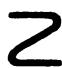
\includegraphics[keepaspectratio]{images/part002_8e27f267.jpg}}

若扩张 M 在 K 上可分，它在 L 上未必可分（但参见 V，第124页，推论3）。例如，若 p 是一个素数，则有理分式域 \(\mathbf{F}_{p}(\mathbf{X})\) （域 \(F_{p}\) 上一个未定元 X 的）在 \(F_{p}\) 上是可分的（V，第121页，命题6），但它是 \(\mathbf{F}_{p}(\mathbf{X}^{p})\) 的一个 p-根式代数扩张；特别地， \(\mathbf{F}_{p}(\mathbf{X})\) 在 \(\mathbf{F}_{p}(\mathbf{X}^{p})\) 上不是可分的。

稍后（V，第137页，命题5）我们将研究复合扩张的可分性。
